\documentclass{book}
\usepackage[a4paper,top=2.5cm,bottom=2.5cm,left=2.5cm,right=2.5cm]{geometry}
\usepackage{makeidx}
\usepackage{natbib}
\usepackage{graphicx}
\usepackage{multicol}
\usepackage{float}
\usepackage{listings}
\usepackage{color}
\usepackage{ifthen}
\usepackage[table]{xcolor}
\usepackage{textcomp}
\usepackage{alltt}
\usepackage{ifpdf}
\ifpdf
\usepackage[pdftex,
            pagebackref=true,
            colorlinks=true,
            linkcolor=blue,
            unicode
           ]{hyperref}
\else
\usepackage[ps2pdf,
            pagebackref=true,
            colorlinks=true,
            linkcolor=blue,
            unicode
           ]{hyperref}
\usepackage{pspicture}
\fi
\usepackage[utf8]{inputenc}
\usepackage{mathptmx}
\usepackage[scaled=.90]{helvet}
\usepackage{courier}
\usepackage{sectsty}
\usepackage{amssymb}
\usepackage[titles]{tocloft}
\usepackage{doxygen}
\lstset{language=C++,inputencoding=utf8,basicstyle=\footnotesize,breaklines=true,breakatwhitespace=true,tabsize=8,numbers=left }
\makeindex
\setcounter{tocdepth}{3}
\renewcommand{\footrulewidth}{0.4pt}
\renewcommand{\familydefault}{\sfdefault}
\hfuzz=15pt
\setlength{\emergencystretch}{15pt}
\hbadness=750
\tolerance=750
\begin{document}
\hypersetup{pageanchor=false,citecolor=blue}
\begin{titlepage}
\vspace*{7cm}
\begin{center}
{\Large My Project }\\
\vspace*{1cm}
{\large Generated by Doxygen 1.8.1.2}\\
\vspace*{0.5cm}
{\small Thu Dec 12 2013 15:03:51}\\
\end{center}
\end{titlepage}
\clearemptydoublepage
\pagenumbering{roman}
\tableofcontents
\clearemptydoublepage
\pagenumbering{arabic}
\hypersetup{pageanchor=true,citecolor=blue}
\chapter{Bug List}
\label{bug}
\hypertarget{bug}{}

\begin{DoxyRefList}
\item[\label{bug__bug000001}%
\hypertarget{bug__bug000001}{}%
Namespace \hyperlink{namespaceUi}{Ui} ]Il manque la gestion des visiteurs. \begin{DoxyCopyright}{Copyright}
G\-N\-U Public License. 
\end{DoxyCopyright}

\end{DoxyRefList}
\chapter{Namespace Index}
\section{Namespace List}
Here is a list of all documented namespaces with brief descriptions\-:\begin{DoxyCompactList}
\item\contentsline{section}{\hyperlink{namespaceUi}{Ui} \\*Classe \hyperlink{classUi_1_1Dialog}{Dialog} Cette classe créé la fenêtre de connexion }{\pageref{namespaceUi}}{}
\end{DoxyCompactList}

\chapter{Class Index}
\section{Class Hierarchy}
This inheritance list is sorted roughly, but not completely, alphabetically\-:\begin{DoxyCompactList}
\item \contentsline{section}{Dialog}{\pageref{classDialog}}{}
\item \contentsline{section}{Dialog\-Ajout\-Medicament}{\pageref{classDialogAjoutMedicament}}{}
\item \contentsline{section}{Dialog\-Ajout\-Praticien}{\pageref{classDialogAjoutPraticien}}{}
\item \contentsline{section}{Dialog\-Confirm\-Ajout}{\pageref{classDialogConfirmAjout}}{}
\item \contentsline{section}{Dialog\-Modif\-Medicament}{\pageref{classDialogModifMedicament}}{}
\item \contentsline{section}{Dialog\-Modif\-Praticien}{\pageref{classDialogModifPraticien}}{}
\item \contentsline{section}{Main\-Window}{\pageref{classMainWindow}}{}
\item \contentsline{section}{Ui\-\_\-\-Dialog}{\pageref{classUi__Dialog}}{}
\begin{DoxyCompactList}
\item \contentsline{section}{Ui\-:\-:Dialog}{\pageref{classUi_1_1Dialog}}{}
\end{DoxyCompactList}
\item \contentsline{section}{Ui\-\_\-\-Dialog\-Ajout\-Medicament}{\pageref{classUi__DialogAjoutMedicament}}{}
\begin{DoxyCompactList}
\item \contentsline{section}{Ui\-:\-:Dialog\-Ajout\-Medicament}{\pageref{classUi_1_1DialogAjoutMedicament}}{}
\end{DoxyCompactList}
\item \contentsline{section}{Ui\-\_\-\-Dialog\-Ajout\-Praticien}{\pageref{classUi__DialogAjoutPraticien}}{}
\begin{DoxyCompactList}
\item \contentsline{section}{Ui\-:\-:Dialog\-Ajout\-Praticien}{\pageref{classUi_1_1DialogAjoutPraticien}}{}
\end{DoxyCompactList}
\item \contentsline{section}{Ui\-\_\-\-Dialog\-Confirm\-Ajout}{\pageref{classUi__DialogConfirmAjout}}{}
\begin{DoxyCompactList}
\item \contentsline{section}{Ui\-:\-:Dialog\-Confirm\-Ajout}{\pageref{classUi_1_1DialogConfirmAjout}}{}
\end{DoxyCompactList}
\item \contentsline{section}{Ui\-\_\-\-Dialog\-Modif\-Medicament}{\pageref{classUi__DialogModifMedicament}}{}
\begin{DoxyCompactList}
\item \contentsline{section}{Ui\-:\-:Dialog\-Modif\-Medicament}{\pageref{classUi_1_1DialogModifMedicament}}{}
\end{DoxyCompactList}
\item \contentsline{section}{Ui\-\_\-\-Dialog\-Modif\-Praticien}{\pageref{classUi__DialogModifPraticien}}{}
\begin{DoxyCompactList}
\item \contentsline{section}{Ui\-:\-:Dialog\-Modif\-Praticien}{\pageref{classUi_1_1DialogModifPraticien}}{}
\end{DoxyCompactList}
\item \contentsline{section}{Ui\-\_\-\-Main\-Window}{\pageref{classUi__MainWindow}}{}
\begin{DoxyCompactList}
\item \contentsline{section}{Ui\-:\-:Main\-Window}{\pageref{classUi_1_1MainWindow}}{}
\end{DoxyCompactList}
\end{DoxyCompactList}

\chapter{Class Index}
\section{Class List}
Here are the classes, structs, unions and interfaces with brief descriptions\-:\begin{DoxyCompactList}
\item\contentsline{section}{\hyperlink{classDialog}{Dialog} }{\pageref{classDialog}}{}
\item\contentsline{section}{\hyperlink{classUi_1_1Dialog}{Ui\-::\-Dialog} }{\pageref{classUi_1_1Dialog}}{}
\item\contentsline{section}{\hyperlink{classDialogAjoutMedicament}{Dialog\-Ajout\-Medicament} }{\pageref{classDialogAjoutMedicament}}{}
\item\contentsline{section}{\hyperlink{classUi_1_1DialogAjoutMedicament}{Ui\-::\-Dialog\-Ajout\-Medicament} }{\pageref{classUi_1_1DialogAjoutMedicament}}{}
\item\contentsline{section}{\hyperlink{classDialogAjoutPraticien}{Dialog\-Ajout\-Praticien} }{\pageref{classDialogAjoutPraticien}}{}
\item\contentsline{section}{\hyperlink{classUi_1_1DialogAjoutPraticien}{Ui\-::\-Dialog\-Ajout\-Praticien} }{\pageref{classUi_1_1DialogAjoutPraticien}}{}
\item\contentsline{section}{\hyperlink{classDialogConfirmAjout}{Dialog\-Confirm\-Ajout} }{\pageref{classDialogConfirmAjout}}{}
\item\contentsline{section}{\hyperlink{classUi_1_1DialogConfirmAjout}{Ui\-::\-Dialog\-Confirm\-Ajout} }{\pageref{classUi_1_1DialogConfirmAjout}}{}
\item\contentsline{section}{\hyperlink{classUi_1_1DialogModifMedicament}{Ui\-::\-Dialog\-Modif\-Medicament} }{\pageref{classUi_1_1DialogModifMedicament}}{}
\item\contentsline{section}{\hyperlink{classDialogModifMedicament}{Dialog\-Modif\-Medicament} }{\pageref{classDialogModifMedicament}}{}
\item\contentsline{section}{\hyperlink{classUi_1_1DialogModifPraticien}{Ui\-::\-Dialog\-Modif\-Praticien} }{\pageref{classUi_1_1DialogModifPraticien}}{}
\item\contentsline{section}{\hyperlink{classDialogModifPraticien}{Dialog\-Modif\-Praticien} }{\pageref{classDialogModifPraticien}}{}
\item\contentsline{section}{\hyperlink{classUi_1_1MainWindow}{Ui\-::\-Main\-Window} }{\pageref{classUi_1_1MainWindow}}{}
\item\contentsline{section}{\hyperlink{classMainWindow}{Main\-Window} }{\pageref{classMainWindow}}{}
\item\contentsline{section}{\hyperlink{classUi__Dialog}{Ui\-\_\-\-Dialog} }{\pageref{classUi__Dialog}}{}
\item\contentsline{section}{\hyperlink{classUi__DialogAjoutMedicament}{Ui\-\_\-\-Dialog\-Ajout\-Medicament} }{\pageref{classUi__DialogAjoutMedicament}}{}
\item\contentsline{section}{\hyperlink{classUi__DialogAjoutPraticien}{Ui\-\_\-\-Dialog\-Ajout\-Praticien} }{\pageref{classUi__DialogAjoutPraticien}}{}
\item\contentsline{section}{\hyperlink{classUi__DialogConfirmAjout}{Ui\-\_\-\-Dialog\-Confirm\-Ajout} }{\pageref{classUi__DialogConfirmAjout}}{}
\item\contentsline{section}{\hyperlink{classUi__DialogModifMedicament}{Ui\-\_\-\-Dialog\-Modif\-Medicament} }{\pageref{classUi__DialogModifMedicament}}{}
\item\contentsline{section}{\hyperlink{classUi__DialogModifPraticien}{Ui\-\_\-\-Dialog\-Modif\-Praticien} }{\pageref{classUi__DialogModifPraticien}}{}
\item\contentsline{section}{\hyperlink{classUi__MainWindow}{Ui\-\_\-\-Main\-Window} }{\pageref{classUi__MainWindow}}{}
\end{DoxyCompactList}

\chapter{Namespace Documentation}
\hypertarget{namespaceUi}{\section{Ui Namespace Reference}
\label{namespaceUi}\index{Ui@{Ui}}
}


Classe \hyperlink{classUi_1_1Dialog}{Dialog} Cette classe créé la fenêtre de connexion.  


\subsection*{Classes}
\begin{DoxyCompactItemize}
\item 
class \hyperlink{classUi_1_1Dialog}{Dialog}
\item 
class \hyperlink{classUi_1_1DialogAjoutMedicament}{Dialog\-Ajout\-Medicament}
\item 
class \hyperlink{classUi_1_1DialogAjoutPraticien}{Dialog\-Ajout\-Praticien}
\item 
class \hyperlink{classUi_1_1DialogConfirmAjout}{Dialog\-Confirm\-Ajout}
\item 
class \hyperlink{classUi_1_1DialogModifMedicament}{Dialog\-Modif\-Medicament}
\item 
class \hyperlink{classUi_1_1DialogModifPraticien}{Dialog\-Modif\-Praticien}
\item 
class \hyperlink{classUi_1_1MainWindow}{Main\-Window}
\end{DoxyCompactItemize}


\subsection{Detailed Description}
Classe \hyperlink{classUi_1_1Dialog}{Dialog} Cette classe créé la fenêtre de connexion. Back Office G\-S\-B.

Classe \hyperlink{classUi_1_1DialogAjoutPraticien}{Dialog\-Ajout\-Praticien} Cette classe créé la fenêtre d'ajout de praticien.

Classe \hyperlink{classUi_1_1DialogAjoutMedicament}{Dialog\-Ajout\-Medicament} Cette classe créé la fenêtre d'ajout de médicament.

\begin{DoxyAuthor}{Author}
Alexandre Delienne 
\end{DoxyAuthor}
\begin{DoxyVersion}{Version}
1.\-0 
\end{DoxyVersion}
\begin{DoxyDate}{Date}
5/12/2013 
\end{DoxyDate}
\begin{DoxyCopyright}{Copyright}
G\-N\-U Public License.
\end{DoxyCopyright}
Application permettant la vue, la modification et la suppression des médicaments, praticiens et visiteur pour la société G\-S\-B. \begin{DoxyAuthor}{Author}
Alexandre Delienne 
\end{DoxyAuthor}
\begin{DoxyVersion}{Version}
0.\-1a 
\end{DoxyVersion}
\begin{DoxyDate}{Date}
6/12/2013 
\end{DoxyDate}
\begin{DoxyRefDesc}{Bug}
\item[\hyperlink{bug__bug000001}{Bug}]Il manque la gestion des visiteurs. \begin{DoxyCopyright}{Copyright}
G\-N\-U Public License. 
\end{DoxyCopyright}
\end{DoxyRefDesc}

\chapter{Class Documentation}
\hypertarget{classDialog}{\section{Dialog Class Reference}
\label{classDialog}\index{Dialog@{Dialog}}
}
\subsection*{Public Member Functions}
\begin{DoxyCompactItemize}
\item 
\hypertarget{classDialog_acfa2063f9f962d394c6a645b6e7e08d8}{{\bfseries Dialog} (Q\-Widget $\ast$parent=0)}\label{classDialog_acfa2063f9f962d394c6a645b6e7e08d8}

\end{DoxyCompactItemize}


The documentation for this class was generated from the following files\-:\begin{DoxyCompactItemize}
\item 
dialog.\-h\item 
dialog.\-cpp\end{DoxyCompactItemize}

\hypertarget{classUi_1_1Dialog}{\section{Ui\-:\-:Dialog Class Reference}
\label{classUi_1_1Dialog}\index{Ui\-::\-Dialog@{Ui\-::\-Dialog}}
}
Inheritance diagram for Ui\-:\-:Dialog\-:\begin{figure}[H]
\begin{center}
\leavevmode
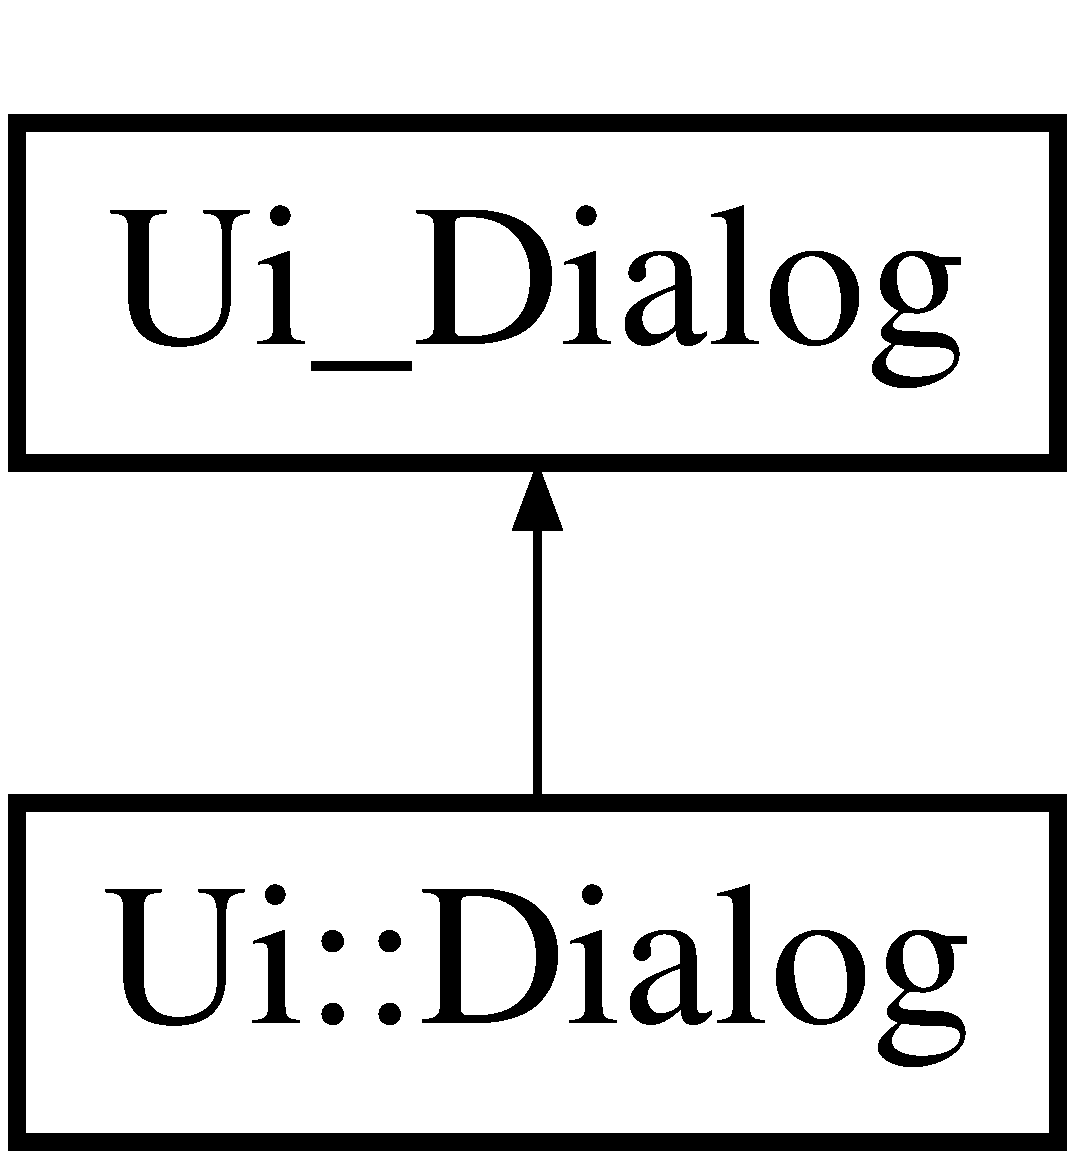
\includegraphics[height=2.000000cm]{classUi_1_1Dialog}
\end{center}
\end{figure}
\subsection*{Additional Inherited Members}


The documentation for this class was generated from the following file\-:\begin{DoxyCompactItemize}
\item 
ui\-\_\-dialog.\-h\end{DoxyCompactItemize}

\hypertarget{classDialogAjoutMedicament}{\section{Dialog\-Ajout\-Medicament Class Reference}
\label{classDialogAjoutMedicament}\index{Dialog\-Ajout\-Medicament@{Dialog\-Ajout\-Medicament}}
}
\subsection*{Public Member Functions}
\begin{DoxyCompactItemize}
\item 
\hypertarget{classDialogAjoutMedicament_a9c1095e61714c053e004c73dd5ba0565}{{\bfseries Dialog\-Ajout\-Medicament} (Q\-Widget $\ast$parent=0)}\label{classDialogAjoutMedicament_a9c1095e61714c053e004c73dd5ba0565}

\end{DoxyCompactItemize}


The documentation for this class was generated from the following files\-:\begin{DoxyCompactItemize}
\item 
dialogajoutmedicament.\-h\item 
dialogajoutmedicament.\-cpp\end{DoxyCompactItemize}

\hypertarget{classUi_1_1DialogAjoutMedicament}{\section{Ui\-:\-:Dialog\-Ajout\-Medicament Class Reference}
\label{classUi_1_1DialogAjoutMedicament}\index{Ui\-::\-Dialog\-Ajout\-Medicament@{Ui\-::\-Dialog\-Ajout\-Medicament}}
}
Inheritance diagram for Ui\-:\-:Dialog\-Ajout\-Medicament\-:\begin{figure}[H]
\begin{center}
\leavevmode
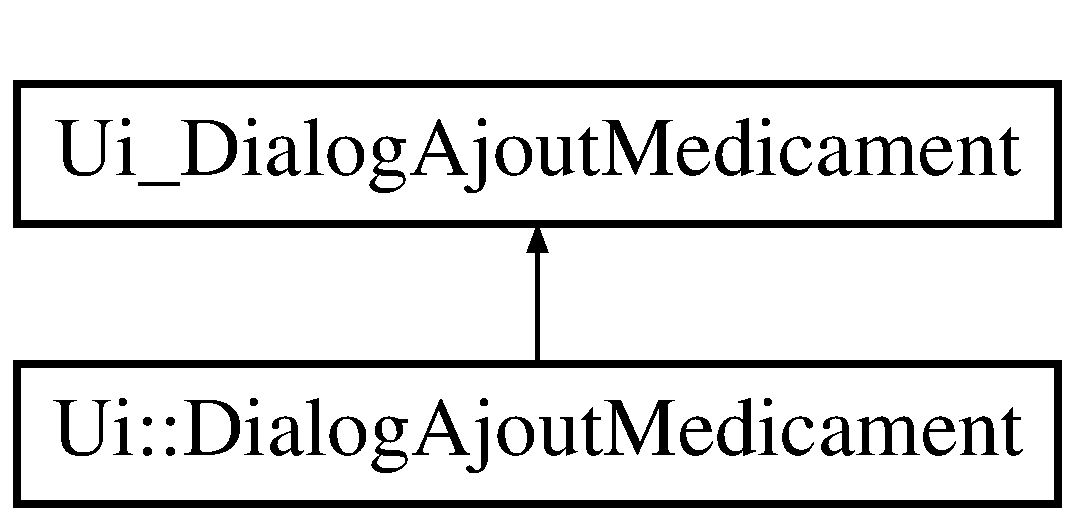
\includegraphics[height=2.000000cm]{classUi_1_1DialogAjoutMedicament}
\end{center}
\end{figure}
\subsection*{Additional Inherited Members}


The documentation for this class was generated from the following file\-:\begin{DoxyCompactItemize}
\item 
ui\-\_\-dialogajoutmedicament.\-h\end{DoxyCompactItemize}

\hypertarget{classDialogAjoutPraticien}{\section{Dialog\-Ajout\-Praticien Class Reference}
\label{classDialogAjoutPraticien}\index{Dialog\-Ajout\-Praticien@{Dialog\-Ajout\-Praticien}}
}
\subsection*{Public Member Functions}
\begin{DoxyCompactItemize}
\item 
\hypertarget{classDialogAjoutPraticien_a92e3f7a1059f169e3b88d9fb33b008fc}{{\bfseries Dialog\-Ajout\-Praticien} (Q\-Widget $\ast$parent=0)}\label{classDialogAjoutPraticien_a92e3f7a1059f169e3b88d9fb33b008fc}

\end{DoxyCompactItemize}


The documentation for this class was generated from the following files\-:\begin{DoxyCompactItemize}
\item 
dialogajoutpraticien.\-h\item 
dialogajoutpraticien.\-cpp\end{DoxyCompactItemize}

\hypertarget{classUi_1_1DialogAjoutPraticien}{\section{Ui\-:\-:Dialog\-Ajout\-Praticien Class Reference}
\label{classUi_1_1DialogAjoutPraticien}\index{Ui\-::\-Dialog\-Ajout\-Praticien@{Ui\-::\-Dialog\-Ajout\-Praticien}}
}
Inheritance diagram for Ui\-:\-:Dialog\-Ajout\-Praticien\-:\begin{figure}[H]
\begin{center}
\leavevmode
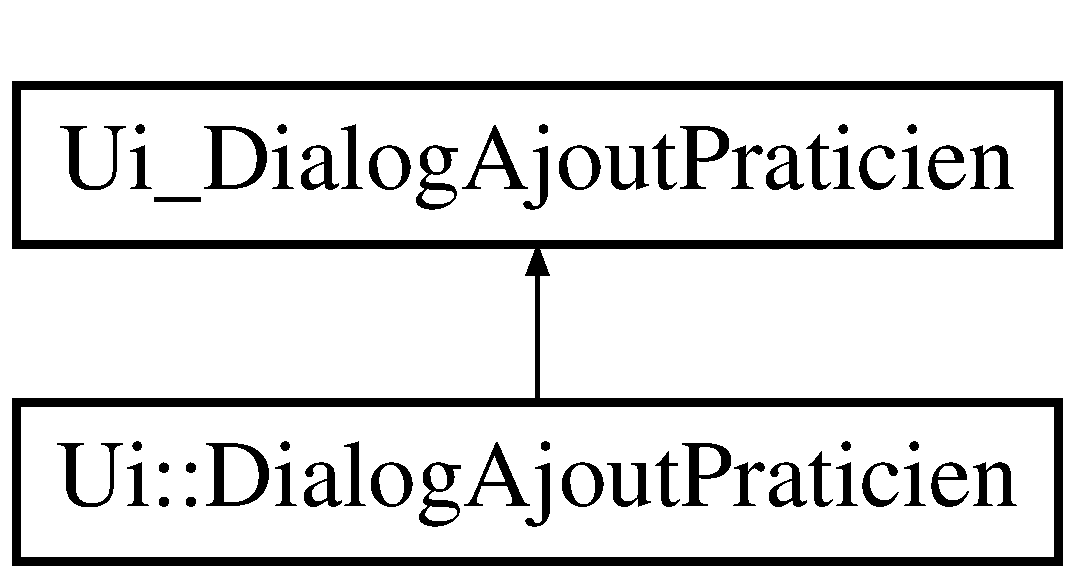
\includegraphics[height=2.000000cm]{classUi_1_1DialogAjoutPraticien}
\end{center}
\end{figure}
\subsection*{Additional Inherited Members}


The documentation for this class was generated from the following file\-:\begin{DoxyCompactItemize}
\item 
ui\-\_\-dialogajoutpraticien.\-h\end{DoxyCompactItemize}

\hypertarget{classDialogConfirmAjout}{\section{Dialog\-Confirm\-Ajout Class Reference}
\label{classDialogConfirmAjout}\index{Dialog\-Confirm\-Ajout@{Dialog\-Confirm\-Ajout}}
}
\subsection*{Public Member Functions}
\begin{DoxyCompactItemize}
\item 
\hypertarget{classDialogConfirmAjout_a6c1e384266f1075aba773cf3f09c0d89}{{\bfseries Dialog\-Confirm\-Ajout} (Q\-Widget $\ast$parent=0)}\label{classDialogConfirmAjout_a6c1e384266f1075aba773cf3f09c0d89}

\item 
\hypertarget{classDialogConfirmAjout_a8d51c08ee586615094be978ea4fecd9a}{void {\bfseries affiche} (Q\-String)}\label{classDialogConfirmAjout_a8d51c08ee586615094be978ea4fecd9a}

\end{DoxyCompactItemize}


The documentation for this class was generated from the following files\-:\begin{DoxyCompactItemize}
\item 
dialogconfirmajout.\-h\item 
dialogconfirmajout.\-cpp\end{DoxyCompactItemize}

\hypertarget{classUi_1_1DialogConfirmAjout}{\section{Ui\-:\-:Dialog\-Confirm\-Ajout Class Reference}
\label{classUi_1_1DialogConfirmAjout}\index{Ui\-::\-Dialog\-Confirm\-Ajout@{Ui\-::\-Dialog\-Confirm\-Ajout}}
}
Inheritance diagram for Ui\-:\-:Dialog\-Confirm\-Ajout\-:\begin{figure}[H]
\begin{center}
\leavevmode
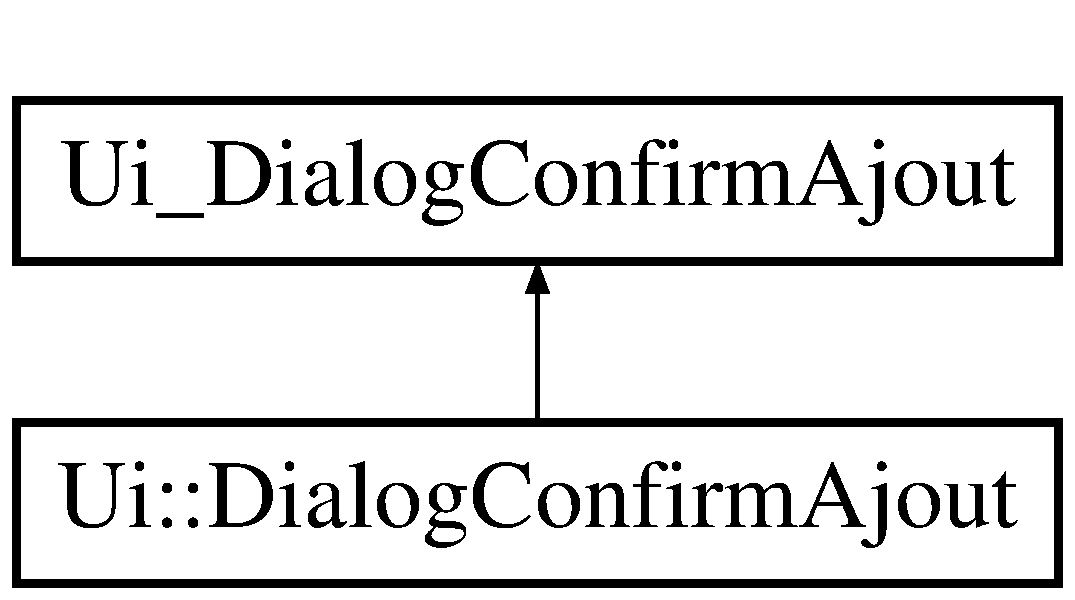
\includegraphics[height=2.000000cm]{classUi_1_1DialogConfirmAjout}
\end{center}
\end{figure}
\subsection*{Additional Inherited Members}


The documentation for this class was generated from the following file\-:\begin{DoxyCompactItemize}
\item 
ui\-\_\-dialogconfirmajout.\-h\end{DoxyCompactItemize}

\hypertarget{classUi_1_1DialogModifMedicament}{\section{Ui\-:\-:Dialog\-Modif\-Medicament Class Reference}
\label{classUi_1_1DialogModifMedicament}\index{Ui\-::\-Dialog\-Modif\-Medicament@{Ui\-::\-Dialog\-Modif\-Medicament}}
}
Inheritance diagram for Ui\-:\-:Dialog\-Modif\-Medicament\-:\begin{figure}[H]
\begin{center}
\leavevmode
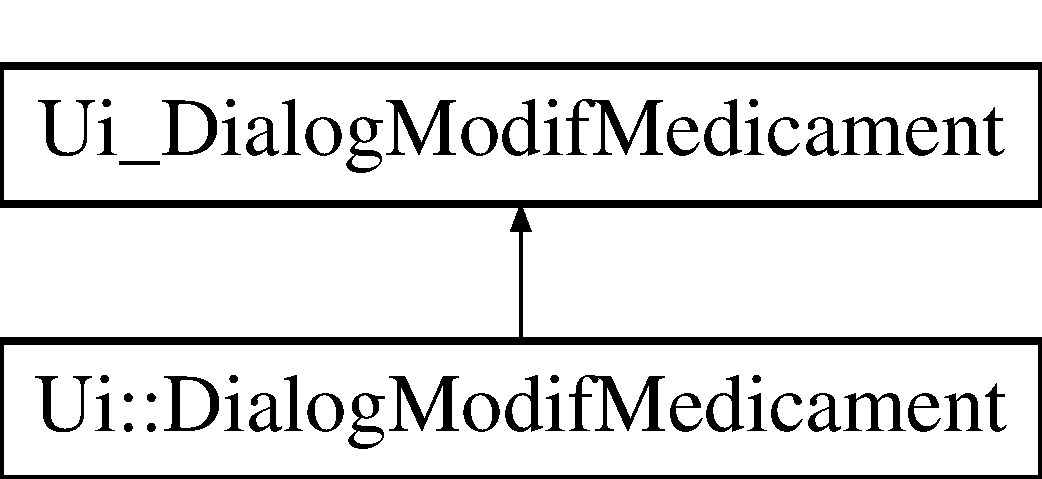
\includegraphics[height=2.000000cm]{classUi_1_1DialogModifMedicament}
\end{center}
\end{figure}
\subsection*{Additional Inherited Members}


The documentation for this class was generated from the following file\-:\begin{DoxyCompactItemize}
\item 
ui\-\_\-dialogmodifmedicament.\-h\end{DoxyCompactItemize}

\hypertarget{classDialogModifMedicament}{\section{Dialog\-Modif\-Medicament Class Reference}
\label{classDialogModifMedicament}\index{Dialog\-Modif\-Medicament@{Dialog\-Modif\-Medicament}}
}
\subsection*{Public Member Functions}
\begin{DoxyCompactItemize}
\item 
\hypertarget{classDialogModifMedicament_ae00955325ab722261f6ba310fe09369c}{{\bfseries Dialog\-Modif\-Medicament} (Q\-Widget $\ast$parent=0)}\label{classDialogModifMedicament_ae00955325ab722261f6ba310fe09369c}

\end{DoxyCompactItemize}


The documentation for this class was generated from the following files\-:\begin{DoxyCompactItemize}
\item 
dialogmodifmedicament.\-h\item 
dialogmodifmedicament.\-cpp\end{DoxyCompactItemize}

\hypertarget{classUi_1_1DialogModifPraticien}{\section{Ui\-:\-:Dialog\-Modif\-Praticien Class Reference}
\label{classUi_1_1DialogModifPraticien}\index{Ui\-::\-Dialog\-Modif\-Praticien@{Ui\-::\-Dialog\-Modif\-Praticien}}
}
Inheritance diagram for Ui\-:\-:Dialog\-Modif\-Praticien\-:\begin{figure}[H]
\begin{center}
\leavevmode
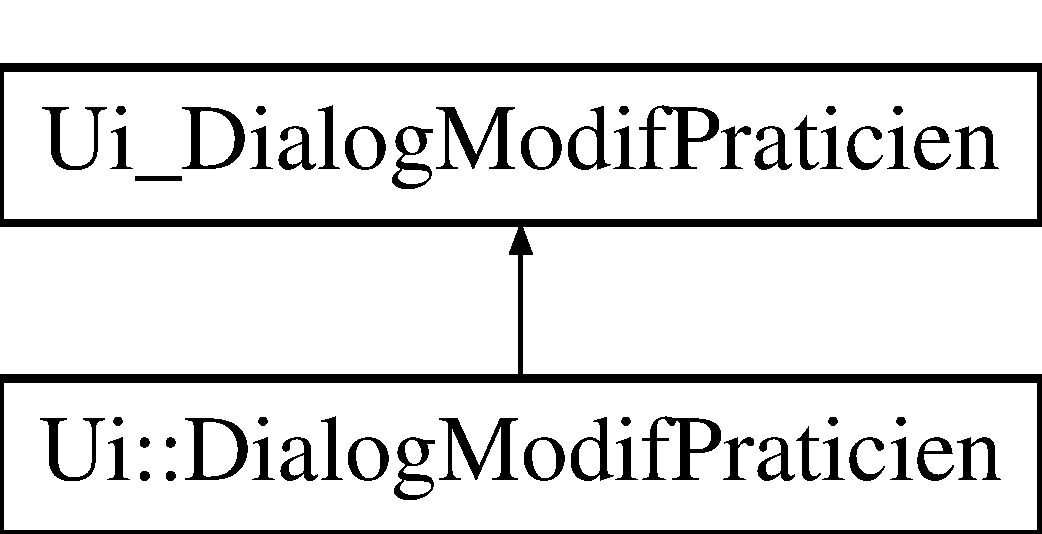
\includegraphics[height=2.000000cm]{classUi_1_1DialogModifPraticien}
\end{center}
\end{figure}
\subsection*{Additional Inherited Members}


The documentation for this class was generated from the following file\-:\begin{DoxyCompactItemize}
\item 
ui\-\_\-dialogmodifpraticien.\-h\end{DoxyCompactItemize}

\hypertarget{classDialogModifPraticien}{\section{Dialog\-Modif\-Praticien Class Reference}
\label{classDialogModifPraticien}\index{Dialog\-Modif\-Praticien@{Dialog\-Modif\-Praticien}}
}
\subsection*{Public Member Functions}
\begin{DoxyCompactItemize}
\item 
\hypertarget{classDialogModifPraticien_ad7dd372c86f700ecf2c39b9d3804a2d3}{{\bfseries Dialog\-Modif\-Praticien} (Q\-Widget $\ast$parent=0)}\label{classDialogModifPraticien_ad7dd372c86f700ecf2c39b9d3804a2d3}

\end{DoxyCompactItemize}


The documentation for this class was generated from the following files\-:\begin{DoxyCompactItemize}
\item 
dialogmodifpraticien.\-h\item 
dialogmodifpraticien.\-cpp\end{DoxyCompactItemize}

\hypertarget{classUi_1_1MainWindow}{\section{Ui\-:\-:Main\-Window Class Reference}
\label{classUi_1_1MainWindow}\index{Ui\-::\-Main\-Window@{Ui\-::\-Main\-Window}}
}
Inheritance diagram for Ui\-:\-:Main\-Window\-:\begin{figure}[H]
\begin{center}
\leavevmode
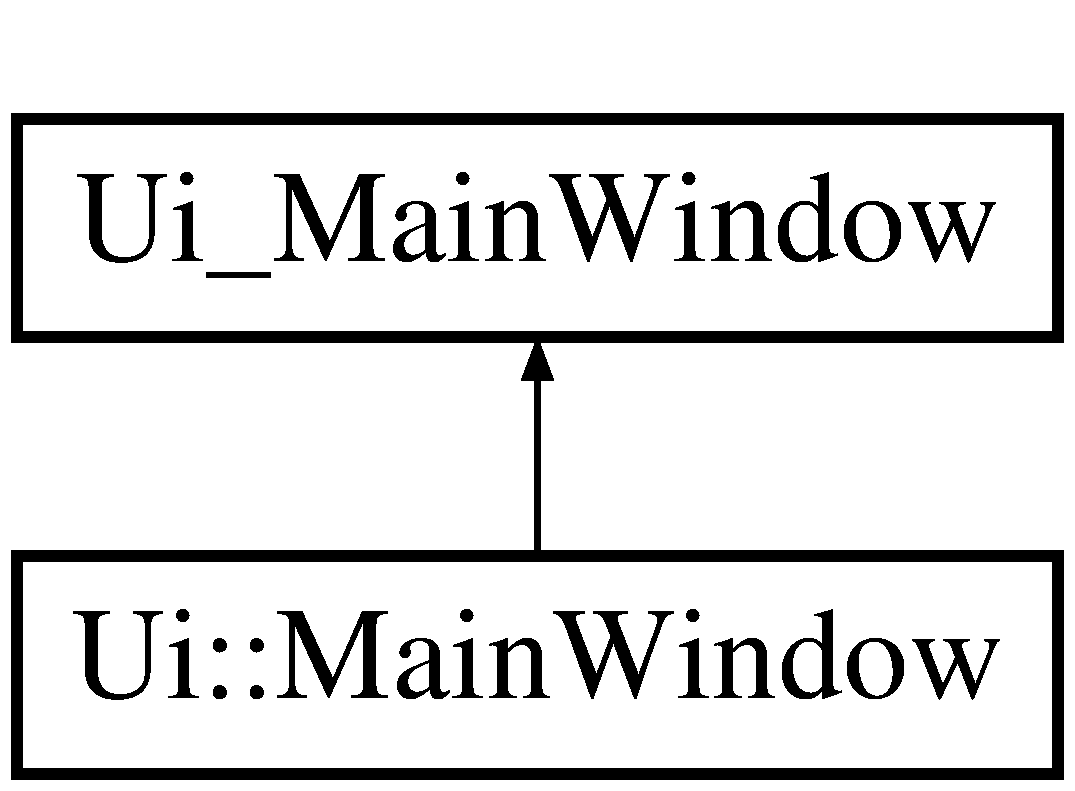
\includegraphics[height=2.000000cm]{classUi_1_1MainWindow}
\end{center}
\end{figure}
\subsection*{Additional Inherited Members}


The documentation for this class was generated from the following file\-:\begin{DoxyCompactItemize}
\item 
ui\-\_\-mainwindow.\-h\end{DoxyCompactItemize}

\hypertarget{classMainWindow}{\section{Main\-Window Class Reference}
\label{classMainWindow}\index{Main\-Window@{Main\-Window}}
}
\subsection*{Public Member Functions}
\begin{DoxyCompactItemize}
\item 
\hyperlink{classMainWindow_a8b244be8b7b7db1b08de2a2acb9409db}{Main\-Window} (Q\-Widget $\ast$parent=0)
\begin{DoxyCompactList}\small\item\em \hyperlink{classMainWindow}{Main\-Window}. \end{DoxyCompactList}\item 
\hypertarget{classMainWindow_a16abc3228e59b5eb189421c08aaac840}{void {\bfseries charge\-Liste\-Medicament} ()}\label{classMainWindow_a16abc3228e59b5eb189421c08aaac840}

\item 
\hypertarget{classMainWindow_a6e9e81db288f845d027aa24926b837aa}{void {\bfseries charge\-Liste\-Praticien} ()}\label{classMainWindow_a6e9e81db288f845d027aa24926b837aa}

\item 
\hypertarget{classMainWindow_aad1e0adee1331df491dff072ce98e663}{void {\bfseries charge\-Liste\-Visiteur} ()}\label{classMainWindow_aad1e0adee1331df491dff072ce98e663}

\item 
\hypertarget{classMainWindow_a24fff6171cd4ade3fedfe3c04e96c8a6}{void {\bfseries chargecombo\-Box\-Famille} ()}\label{classMainWindow_a24fff6171cd4ade3fedfe3c04e96c8a6}

\item 
\hypertarget{classMainWindow_a674ca789f95e94ffaa77db7c9c1ecfe2}{void {\bfseries chargecombo\-Box\-Type} ()}\label{classMainWindow_a674ca789f95e94ffaa77db7c9c1ecfe2}

\item 
\hypertarget{classMainWindow_afedcf0d4d76c575285242f16568b8ca0}{void {\bfseries chargecombo\-Box\-Ville} ()}\label{classMainWindow_afedcf0d4d76c575285242f16568b8ca0}

\item 
\hypertarget{classMainWindow_a88d8712b73cab139199a9fafa9b68279}{void {\bfseries chargecombo\-Box\-Ville2} ()}\label{classMainWindow_a88d8712b73cab139199a9fafa9b68279}

\end{DoxyCompactItemize}
\subsection*{Public Attributes}
\begin{DoxyCompactItemize}
\item 
\hypertarget{classMainWindow_a35466a70ed47252a0191168126a352a5}{\hyperlink{classUi_1_1MainWindow}{Ui\-::\-Main\-Window} $\ast$ {\bfseries ui}}\label{classMainWindow_a35466a70ed47252a0191168126a352a5}

\item 
\hypertarget{classMainWindow_a62a7afcfb541186cc139dd2443059418}{Q\-Vector$<$ Q\-String $>$ {\bfseries vector\-Id\-Famille}}\label{classMainWindow_a62a7afcfb541186cc139dd2443059418}

\item 
\hypertarget{classMainWindow_a1b076047873df46f2d15b17ad05ccdeb}{Q\-Vector$<$ Q\-String $>$ {\bfseries vector\-Id\-Medicament}}\label{classMainWindow_a1b076047873df46f2d15b17ad05ccdeb}

\item 
\hypertarget{classMainWindow_a18373d13428694aad37577326c6faf9b}{Q\-Vector$<$ Q\-String $>$ {\bfseries vector\-Id\-Type}}\label{classMainWindow_a18373d13428694aad37577326c6faf9b}

\item 
\hypertarget{classMainWindow_a010db4d3678ed6ed77fb80f83cd0b47e}{Q\-Vector$<$ Q\-String $>$ {\bfseries vector\-Id\-Ville}}\label{classMainWindow_a010db4d3678ed6ed77fb80f83cd0b47e}

\item 
\hypertarget{classMainWindow_aceca27e15298068686a823768d780f00}{Q\-Vector$<$ Q\-String $>$ {\bfseries vector\-Id\-Praticien}}\label{classMainWindow_aceca27e15298068686a823768d780f00}

\item 
\hypertarget{classMainWindow_ab40795391d054dd03a89d0ec1114e7fc}{Q\-Vector$<$ int $>$ {\bfseries vector\-Id\-Visiteur}}\label{classMainWindow_ab40795391d054dd03a89d0ec1114e7fc}

\end{DoxyCompactItemize}


\subsection{Constructor \& Destructor Documentation}
\hypertarget{classMainWindow_a8b244be8b7b7db1b08de2a2acb9409db}{\index{Main\-Window@{Main\-Window}!Main\-Window@{Main\-Window}}
\index{Main\-Window@{Main\-Window}!MainWindow@{Main\-Window}}
\subsubsection[{Main\-Window}]{\setlength{\rightskip}{0pt plus 5cm}Main\-Window\-::\-Main\-Window (
\begin{DoxyParamCaption}
\item[{Q\-Widget $\ast$}]{parent = {\ttfamily 0}}
\end{DoxyParamCaption}
)\hspace{0.3cm}{\ttfamily [explicit]}}}\label{classMainWindow_a8b244be8b7b7db1b08de2a2acb9409db}


\hyperlink{classMainWindow}{Main\-Window}. 


\begin{DoxyParams}{Parameters}
{\em parent} & \\
\hline
\end{DoxyParams}


The documentation for this class was generated from the following files\-:\begin{DoxyCompactItemize}
\item 
mainwindow.\-h\item 
mainwindow.\-cpp\end{DoxyCompactItemize}

\hypertarget{classUi__Dialog}{\section{Ui\-\_\-\-Dialog Class Reference}
\label{classUi__Dialog}\index{Ui\-\_\-\-Dialog@{Ui\-\_\-\-Dialog}}
}
Inheritance diagram for Ui\-\_\-\-Dialog\-:\begin{figure}[H]
\begin{center}
\leavevmode
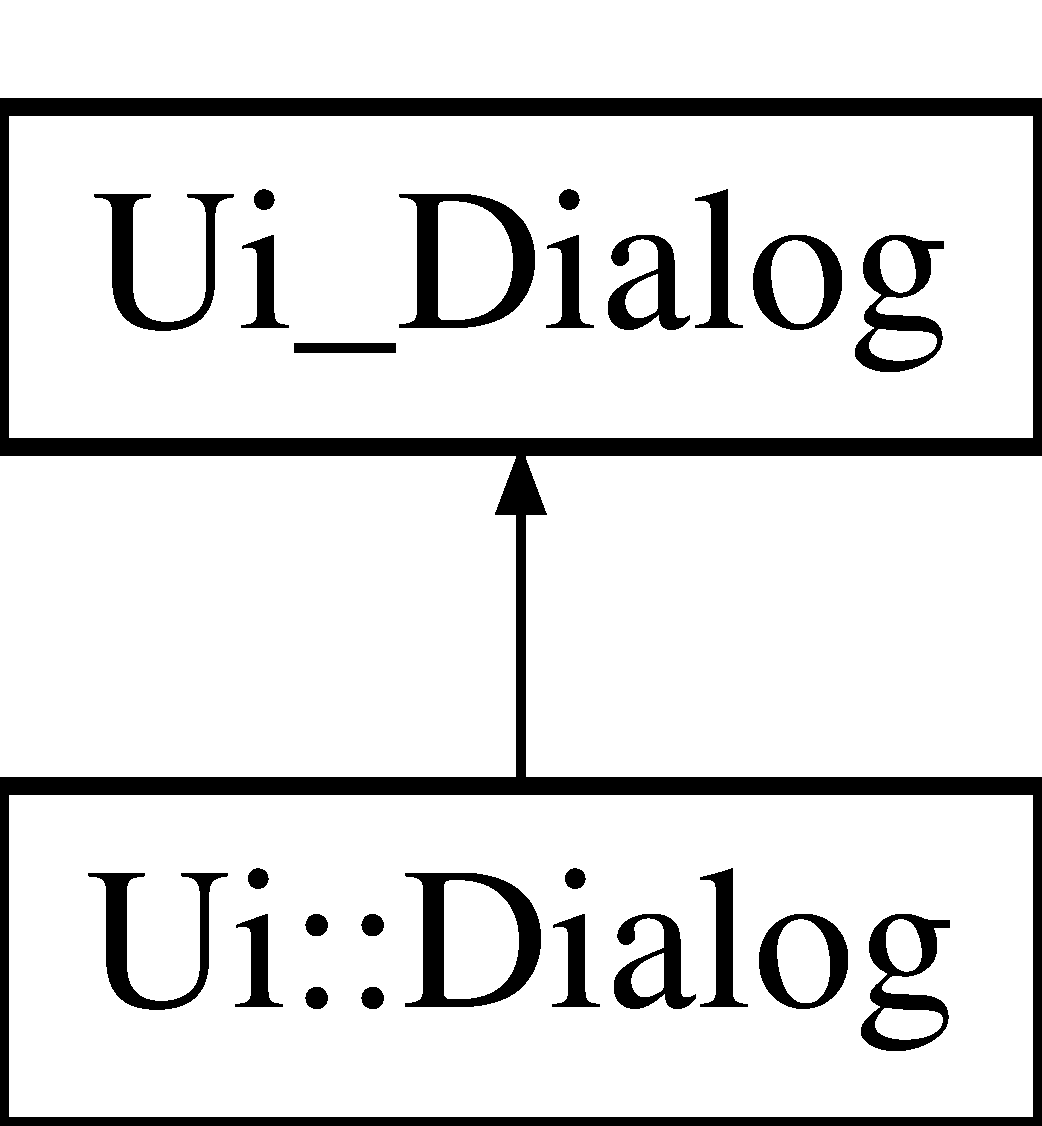
\includegraphics[height=2.000000cm]{classUi__Dialog}
\end{center}
\end{figure}
\subsection*{Public Member Functions}
\begin{DoxyCompactItemize}
\item 
\hypertarget{classUi__Dialog_a4f6a478c3ecdafabffb17b39cb26444a}{void {\bfseries setup\-Ui} (Q\-Dialog $\ast$\hyperlink{classDialog}{Dialog})}\label{classUi__Dialog_a4f6a478c3ecdafabffb17b39cb26444a}

\item 
\hypertarget{classUi__Dialog_afa0ccb6f716ca6178260522a193c250e}{void {\bfseries retranslate\-Ui} (Q\-Dialog $\ast$\hyperlink{classDialog}{Dialog})}\label{classUi__Dialog_afa0ccb6f716ca6178260522a193c250e}

\end{DoxyCompactItemize}
\subsection*{Public Attributes}
\begin{DoxyCompactItemize}
\item 
\hypertarget{classUi__Dialog_a02f973813b741621c5461918b3d9d4bb}{Q\-V\-Box\-Layout $\ast$ {\bfseries vertical\-Layout}}\label{classUi__Dialog_a02f973813b741621c5461918b3d9d4bb}

\item 
\hypertarget{classUi__Dialog_ae66a1da203f045e33d71ed5abd46d2a1}{Q\-H\-Box\-Layout $\ast$ {\bfseries horizontal\-Layout}}\label{classUi__Dialog_ae66a1da203f045e33d71ed5abd46d2a1}

\item 
\hypertarget{classUi__Dialog_a81b52d0f39bcb5cfd3c51f18961c650b}{Q\-Spacer\-Item $\ast$ {\bfseries vertical\-Spacer\-\_\-2}}\label{classUi__Dialog_a81b52d0f39bcb5cfd3c51f18961c650b}

\item 
\hypertarget{classUi__Dialog_a289b49bcdd28408efe2510f029535c2b}{Q\-H\-Box\-Layout $\ast$ {\bfseries horizontal\-Layout\-\_\-2}}\label{classUi__Dialog_a289b49bcdd28408efe2510f029535c2b}

\item 
\hypertarget{classUi__Dialog_affee116cbe843086b0e35ebf998fb67c}{Q\-Spacer\-Item $\ast$ {\bfseries horizontal\-Spacer\-\_\-7}}\label{classUi__Dialog_affee116cbe843086b0e35ebf998fb67c}

\item 
\hypertarget{classUi__Dialog_a41336d41594e8776a81d095e8e4ffc61}{Q\-Grid\-Layout $\ast$ {\bfseries grid\-Layout}}\label{classUi__Dialog_a41336d41594e8776a81d095e8e4ffc61}

\item 
\hypertarget{classUi__Dialog_acfbb1773ba7dc7aa425b0b3b8981686a}{Q\-Label $\ast$ {\bfseries label\-\_\-2}}\label{classUi__Dialog_acfbb1773ba7dc7aa425b0b3b8981686a}

\item 
\hypertarget{classUi__Dialog_abb48dec9e79eb09f978bf5fb062fe7de}{Q\-Line\-Edit $\ast$ {\bfseries line\-Edit\-Login}}\label{classUi__Dialog_abb48dec9e79eb09f978bf5fb062fe7de}

\item 
\hypertarget{classUi__Dialog_a3bb3c83086d124c6e85906f15c8add64}{Q\-Label $\ast$ {\bfseries label\-\_\-3}}\label{classUi__Dialog_a3bb3c83086d124c6e85906f15c8add64}

\item 
\hypertarget{classUi__Dialog_a55903c75c6aaca163f58345785c80eaa}{Q\-Line\-Edit $\ast$ {\bfseries line\-Edit\-Passwd}}\label{classUi__Dialog_a55903c75c6aaca163f58345785c80eaa}

\item 
\hypertarget{classUi__Dialog_a82d8f43c1d5372aa9729796005e784b6}{Q\-Spacer\-Item $\ast$ {\bfseries horizontal\-Spacer\-\_\-8}}\label{classUi__Dialog_a82d8f43c1d5372aa9729796005e784b6}

\item 
\hypertarget{classUi__Dialog_a74941704c736dfff50b9bef8eda12207}{Q\-Spacer\-Item $\ast$ {\bfseries vertical\-Spacer\-\_\-3}}\label{classUi__Dialog_a74941704c736dfff50b9bef8eda12207}

\item 
\hypertarget{classUi__Dialog_acd165ec013acc890cb290ce16b9563f6}{Q\-V\-Box\-Layout $\ast$ {\bfseries vertical\-Layout\-\_\-3}}\label{classUi__Dialog_acd165ec013acc890cb290ce16b9563f6}

\item 
\hypertarget{classUi__Dialog_ab23bf4588fc8ad303dc922ef54138d15}{Q\-H\-Box\-Layout $\ast$ {\bfseries horizontal\-Layout\-\_\-3}}\label{classUi__Dialog_ab23bf4588fc8ad303dc922ef54138d15}

\item 
\hypertarget{classUi__Dialog_a054eeab37d5f8e9a4918d949a44428be}{Q\-Spacer\-Item $\ast$ {\bfseries horizontal\-Spacer\-\_\-3}}\label{classUi__Dialog_a054eeab37d5f8e9a4918d949a44428be}

\item 
\hypertarget{classUi__Dialog_a2d5df2aa7fcc94b3305bb7e34de11253}{Q\-Push\-Button $\ast$ {\bfseries push\-Button\-Connexion}}\label{classUi__Dialog_a2d5df2aa7fcc94b3305bb7e34de11253}

\item 
\hypertarget{classUi__Dialog_af1c89e7936dfd7b410f670b80336b622}{Q\-Spacer\-Item $\ast$ {\bfseries horizontal\-Spacer\-\_\-4}}\label{classUi__Dialog_af1c89e7936dfd7b410f670b80336b622}

\item 
\hypertarget{classUi__Dialog_ac3772f494bf164d526a04feff8314f96}{Q\-H\-Box\-Layout $\ast$ {\bfseries horizontal\-Layout\-\_\-4}}\label{classUi__Dialog_ac3772f494bf164d526a04feff8314f96}

\item 
\hypertarget{classUi__Dialog_a23424803a38ec82be577f3d786a25ee0}{Q\-Spacer\-Item $\ast$ {\bfseries horizontal\-Spacer\-\_\-5}}\label{classUi__Dialog_a23424803a38ec82be577f3d786a25ee0}

\item 
\hypertarget{classUi__Dialog_a78ee6ada2fdeb1c65eb41a8bffc88779}{Q\-Push\-Button $\ast$ {\bfseries push\-Button\-Quitter}}\label{classUi__Dialog_a78ee6ada2fdeb1c65eb41a8bffc88779}

\item 
\hypertarget{classUi__Dialog_aeef14ab9a700a60a517ec304400104e5}{Q\-Spacer\-Item $\ast$ {\bfseries horizontal\-Spacer\-\_\-6}}\label{classUi__Dialog_aeef14ab9a700a60a517ec304400104e5}

\item 
\hypertarget{classUi__Dialog_a5272f4a31affb22b7118cd47e5a96002}{Q\-Spacer\-Item $\ast$ {\bfseries vertical\-Spacer}}\label{classUi__Dialog_a5272f4a31affb22b7118cd47e5a96002}

\end{DoxyCompactItemize}


The documentation for this class was generated from the following file\-:\begin{DoxyCompactItemize}
\item 
ui\-\_\-dialog.\-h\end{DoxyCompactItemize}

\hypertarget{classUi__DialogAjoutMedicament}{\section{Ui\-\_\-\-Dialog\-Ajout\-Medicament Class Reference}
\label{classUi__DialogAjoutMedicament}\index{Ui\-\_\-\-Dialog\-Ajout\-Medicament@{Ui\-\_\-\-Dialog\-Ajout\-Medicament}}
}
Inheritance diagram for Ui\-\_\-\-Dialog\-Ajout\-Medicament\-:\begin{figure}[H]
\begin{center}
\leavevmode
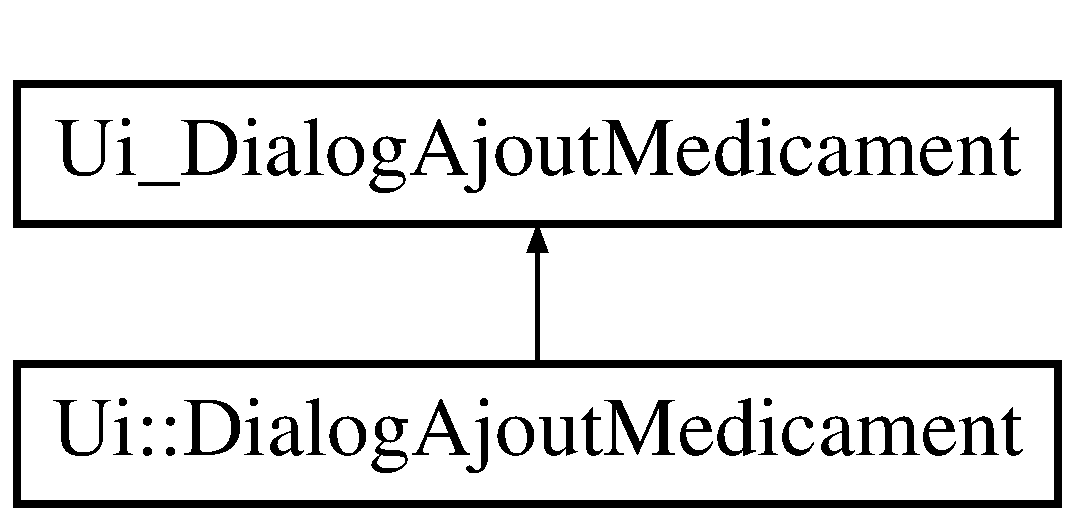
\includegraphics[height=2.000000cm]{classUi__DialogAjoutMedicament}
\end{center}
\end{figure}
\subsection*{Public Member Functions}
\begin{DoxyCompactItemize}
\item 
\hypertarget{classUi__DialogAjoutMedicament_a976edec01e8af86119ce87115c8084b7}{void {\bfseries setup\-Ui} (Q\-Dialog $\ast$\hyperlink{classDialogAjoutMedicament}{Dialog\-Ajout\-Medicament})}\label{classUi__DialogAjoutMedicament_a976edec01e8af86119ce87115c8084b7}

\item 
\hypertarget{classUi__DialogAjoutMedicament_a8c71f7ac08cd1cadc3af5152af427d2e}{void {\bfseries retranslate\-Ui} (Q\-Dialog $\ast$\hyperlink{classDialogAjoutMedicament}{Dialog\-Ajout\-Medicament})}\label{classUi__DialogAjoutMedicament_a8c71f7ac08cd1cadc3af5152af427d2e}

\end{DoxyCompactItemize}
\subsection*{Public Attributes}
\begin{DoxyCompactItemize}
\item 
\hypertarget{classUi__DialogAjoutMedicament_ac80419bc5f8babe6f9fcb5396bb09cb6}{Q\-Grid\-Layout $\ast$ {\bfseries grid\-Layout\-\_\-3}}\label{classUi__DialogAjoutMedicament_ac80419bc5f8babe6f9fcb5396bb09cb6}

\item 
\hypertarget{classUi__DialogAjoutMedicament_a25fa128d6eeb48996d10af963433409d}{Q\-Spacer\-Item $\ast$ {\bfseries vertical\-Spacer\-\_\-2}}\label{classUi__DialogAjoutMedicament_a25fa128d6eeb48996d10af963433409d}

\item 
\hypertarget{classUi__DialogAjoutMedicament_ae540ca6cbfcf171923a9fc0a48fbf2a7}{Q\-Spacer\-Item $\ast$ {\bfseries horizontal\-Spacer\-\_\-6}}\label{classUi__DialogAjoutMedicament_ae540ca6cbfcf171923a9fc0a48fbf2a7}

\item 
\hypertarget{classUi__DialogAjoutMedicament_a3b4dbf7750d1a3d84909bb9c96379d9c}{Q\-Splitter $\ast$ {\bfseries splitter}}\label{classUi__DialogAjoutMedicament_a3b4dbf7750d1a3d84909bb9c96379d9c}

\item 
\hypertarget{classUi__DialogAjoutMedicament_aff7bb6674c572410b4a6ef976d2fae27}{Q\-Widget $\ast$ {\bfseries layout\-Widget}}\label{classUi__DialogAjoutMedicament_aff7bb6674c572410b4a6ef976d2fae27}

\item 
\hypertarget{classUi__DialogAjoutMedicament_a630ad206872bb31c147ddb83e1b16fbd}{Q\-V\-Box\-Layout $\ast$ {\bfseries vertical\-Layout\-\_\-4}}\label{classUi__DialogAjoutMedicament_a630ad206872bb31c147ddb83e1b16fbd}

\item 
\hypertarget{classUi__DialogAjoutMedicament_af44a48bcf0ea1f4262090b4f924a19e3}{Q\-Grid\-Layout $\ast$ {\bfseries grid\-Layout}}\label{classUi__DialogAjoutMedicament_af44a48bcf0ea1f4262090b4f924a19e3}

\item 
\hypertarget{classUi__DialogAjoutMedicament_a27a0e98e09e482b0e197626f31961e04}{Q\-Label $\ast$ {\bfseries label\-Dep\-Legal}}\label{classUi__DialogAjoutMedicament_a27a0e98e09e482b0e197626f31961e04}

\item 
\hypertarget{classUi__DialogAjoutMedicament_a2dbacadd26456cd445f9af92d2bd830d}{Q\-Line\-Edit $\ast$ {\bfseries line\-Edit\-Dep\-Legal}}\label{classUi__DialogAjoutMedicament_a2dbacadd26456cd445f9af92d2bd830d}

\item 
\hypertarget{classUi__DialogAjoutMedicament_a9ccfbba5026bf01b3b837e9d1a987af2}{Q\-Label $\ast$ {\bfseries label\-Nom\-Comm}}\label{classUi__DialogAjoutMedicament_a9ccfbba5026bf01b3b837e9d1a987af2}

\item 
\hypertarget{classUi__DialogAjoutMedicament_a89c38de0f1611097fab64ee7d50613da}{Q\-Line\-Edit $\ast$ {\bfseries line\-Edit\-Nom\-Comm}}\label{classUi__DialogAjoutMedicament_a89c38de0f1611097fab64ee7d50613da}

\item 
\hypertarget{classUi__DialogAjoutMedicament_a5639a19769cf80f6d1e0f5e45bd0a224}{Q\-Label $\ast$ {\bfseries label\-Code\-Famille}}\label{classUi__DialogAjoutMedicament_a5639a19769cf80f6d1e0f5e45bd0a224}

\item 
\hypertarget{classUi__DialogAjoutMedicament_a47ecb9b496caa88466ac79935bf80263}{Q\-Combo\-Box $\ast$ {\bfseries combo\-Box\-Famille\-Ajout}}\label{classUi__DialogAjoutMedicament_a47ecb9b496caa88466ac79935bf80263}

\item 
\hypertarget{classUi__DialogAjoutMedicament_a2b6cfdc1ac1f959d57fcee5d760e2158}{Q\-Label $\ast$ {\bfseries label\-Prix}}\label{classUi__DialogAjoutMedicament_a2b6cfdc1ac1f959d57fcee5d760e2158}

\item 
\hypertarget{classUi__DialogAjoutMedicament_a38d96ddff562db6f42703259ffab7eb2}{Q\-Double\-Spin\-Box $\ast$ {\bfseries double\-Spin\-Box\-Prix}}\label{classUi__DialogAjoutMedicament_a38d96ddff562db6f42703259ffab7eb2}

\item 
\hypertarget{classUi__DialogAjoutMedicament_a5f1aeb12a786cf13351ea8ad0de6ca56}{Q\-H\-Box\-Layout $\ast$ {\bfseries horizontal\-Layout}}\label{classUi__DialogAjoutMedicament_a5f1aeb12a786cf13351ea8ad0de6ca56}

\item 
\hypertarget{classUi__DialogAjoutMedicament_a599d33fb463759e117a9631ed5019f48}{Q\-Spacer\-Item $\ast$ {\bfseries horizontal\-Spacer\-\_\-2}}\label{classUi__DialogAjoutMedicament_a599d33fb463759e117a9631ed5019f48}

\item 
\hypertarget{classUi__DialogAjoutMedicament_af0c83b99175b9580776a3c5b8e92c769}{Q\-Label $\ast$ {\bfseries label\-Logo\-\_\-2}}\label{classUi__DialogAjoutMedicament_af0c83b99175b9580776a3c5b8e92c769}

\item 
\hypertarget{classUi__DialogAjoutMedicament_a1e182e49899fc7917527d18df71d19ff}{Q\-Widget $\ast$ {\bfseries layout\-Widget1}}\label{classUi__DialogAjoutMedicament_a1e182e49899fc7917527d18df71d19ff}

\item 
\hypertarget{classUi__DialogAjoutMedicament_a36289c8b3cea5e8dc2cd664d3a519f71}{Q\-Grid\-Layout $\ast$ {\bfseries grid\-Layout\-\_\-2}}\label{classUi__DialogAjoutMedicament_a36289c8b3cea5e8dc2cd664d3a519f71}

\item 
\hypertarget{classUi__DialogAjoutMedicament_a42a62e35091a4483ec77940827a5e435}{Q\-V\-Box\-Layout $\ast$ {\bfseries vertical\-Layout}}\label{classUi__DialogAjoutMedicament_a42a62e35091a4483ec77940827a5e435}

\item 
\hypertarget{classUi__DialogAjoutMedicament_a35ade5ec787d0351528e574239807d26}{Q\-Label $\ast$ {\bfseries label\-Effets}}\label{classUi__DialogAjoutMedicament_a35ade5ec787d0351528e574239807d26}

\item 
\hypertarget{classUi__DialogAjoutMedicament_aedba34f2af27fc023848bfdcaf2532c2}{Q\-Spacer\-Item $\ast$ {\bfseries vertical\-Spacer}}\label{classUi__DialogAjoutMedicament_aedba34f2af27fc023848bfdcaf2532c2}

\item 
\hypertarget{classUi__DialogAjoutMedicament_affeabd780e5502740d52a7b4ecb06c00}{Q\-V\-Box\-Layout $\ast$ {\bfseries vertical\-Layout\-\_\-2}}\label{classUi__DialogAjoutMedicament_affeabd780e5502740d52a7b4ecb06c00}

\item 
\hypertarget{classUi__DialogAjoutMedicament_a77b00f05cdc9f5731c49cfcb365f796c}{Q\-Label $\ast$ {\bfseries label\-Compo}}\label{classUi__DialogAjoutMedicament_a77b00f05cdc9f5731c49cfcb365f796c}

\item 
\hypertarget{classUi__DialogAjoutMedicament_ae3fa21cae906880384f79128af45b65d}{Q\-Spacer\-Item $\ast$ {\bfseries horizontal\-Spacer\-\_\-4}}\label{classUi__DialogAjoutMedicament_ae3fa21cae906880384f79128af45b65d}

\item 
\hypertarget{classUi__DialogAjoutMedicament_a2be899cf01f5cd3daefbe917910dc985}{Q\-Spacer\-Item $\ast$ {\bfseries vertical\-Spacer\-\_\-4}}\label{classUi__DialogAjoutMedicament_a2be899cf01f5cd3daefbe917910dc985}

\item 
\hypertarget{classUi__DialogAjoutMedicament_a5c50272dc01f7ebf8920cea371700173}{Q\-Text\-Edit $\ast$ {\bfseries text\-Edit\-Compo}}\label{classUi__DialogAjoutMedicament_a5c50272dc01f7ebf8920cea371700173}

\item 
\hypertarget{classUi__DialogAjoutMedicament_a2484e99d62e2ac3009e479661a608533}{Q\-V\-Box\-Layout $\ast$ {\bfseries vertical\-Layout\-\_\-3}}\label{classUi__DialogAjoutMedicament_a2484e99d62e2ac3009e479661a608533}

\item 
\hypertarget{classUi__DialogAjoutMedicament_acb686302fea98c1cb0b8f11a85403c1f}{Q\-Label $\ast$ {\bfseries label\-Contre\-Indic}}\label{classUi__DialogAjoutMedicament_acb686302fea98c1cb0b8f11a85403c1f}

\item 
\hypertarget{classUi__DialogAjoutMedicament_a5f77dabb9b32e96dd23cdd945b6056df}{Q\-Spacer\-Item $\ast$ {\bfseries vertical\-Spacer\-\_\-5}}\label{classUi__DialogAjoutMedicament_a5f77dabb9b32e96dd23cdd945b6056df}

\item 
\hypertarget{classUi__DialogAjoutMedicament_a15d7304e1b782618eab992b5bc1d9dae}{Q\-Text\-Edit $\ast$ {\bfseries text\-Edit\-Contre\-Indic}}\label{classUi__DialogAjoutMedicament_a15d7304e1b782618eab992b5bc1d9dae}

\item 
\hypertarget{classUi__DialogAjoutMedicament_ad45102990d0aff0095d09d62008a6e32}{Q\-Text\-Edit $\ast$ {\bfseries text\-Edit\-Effets}}\label{classUi__DialogAjoutMedicament_ad45102990d0aff0095d09d62008a6e32}

\item 
\hypertarget{classUi__DialogAjoutMedicament_a0c3227cfada2b4d74a5a994185effda7}{Q\-Spacer\-Item $\ast$ {\bfseries horizontal\-Spacer\-\_\-5}}\label{classUi__DialogAjoutMedicament_a0c3227cfada2b4d74a5a994185effda7}

\item 
\hypertarget{classUi__DialogAjoutMedicament_a911d2d0f01bf471fa6503a0f64a273ef}{Q\-H\-Box\-Layout $\ast$ {\bfseries horizontal\-Layout\-\_\-3}}\label{classUi__DialogAjoutMedicament_a911d2d0f01bf471fa6503a0f64a273ef}

\item 
\hypertarget{classUi__DialogAjoutMedicament_aa72f2024e1e0648e1cbd9df0ea2a5465}{Q\-Spacer\-Item $\ast$ {\bfseries horizontal\-Spacer}}\label{classUi__DialogAjoutMedicament_aa72f2024e1e0648e1cbd9df0ea2a5465}

\item 
\hypertarget{classUi__DialogAjoutMedicament_a6f5be158b6e0218526b0c0749c2ccbec}{Q\-Push\-Button $\ast$ {\bfseries push\-Button\-Ok}}\label{classUi__DialogAjoutMedicament_a6f5be158b6e0218526b0c0749c2ccbec}

\item 
\hypertarget{classUi__DialogAjoutMedicament_a5c32fe453bbe66e01a7166aafb08d3da}{Q\-Push\-Button $\ast$ {\bfseries push\-Button\-Annuler}}\label{classUi__DialogAjoutMedicament_a5c32fe453bbe66e01a7166aafb08d3da}

\item 
\hypertarget{classUi__DialogAjoutMedicament_a07c44d8021a462833370f816b7587112}{Q\-Spacer\-Item $\ast$ {\bfseries vertical\-Spacer\-\_\-3}}\label{classUi__DialogAjoutMedicament_a07c44d8021a462833370f816b7587112}

\end{DoxyCompactItemize}


The documentation for this class was generated from the following file\-:\begin{DoxyCompactItemize}
\item 
ui\-\_\-dialogajoutmedicament.\-h\end{DoxyCompactItemize}

\hypertarget{classUi__DialogAjoutPraticien}{\section{Ui\-\_\-\-Dialog\-Ajout\-Praticien Class Reference}
\label{classUi__DialogAjoutPraticien}\index{Ui\-\_\-\-Dialog\-Ajout\-Praticien@{Ui\-\_\-\-Dialog\-Ajout\-Praticien}}
}
Inheritance diagram for Ui\-\_\-\-Dialog\-Ajout\-Praticien\-:\begin{figure}[H]
\begin{center}
\leavevmode
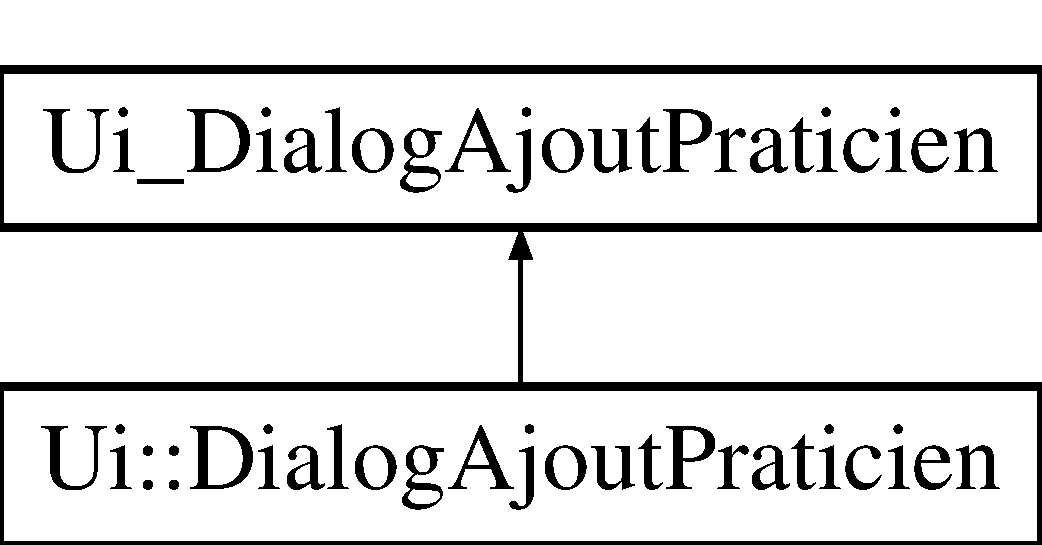
\includegraphics[height=2.000000cm]{classUi__DialogAjoutPraticien}
\end{center}
\end{figure}
\subsection*{Public Member Functions}
\begin{DoxyCompactItemize}
\item 
\hypertarget{classUi__DialogAjoutPraticien_a680faa38056bf525d0f469682c592241}{void {\bfseries setup\-Ui} (Q\-Dialog $\ast$\hyperlink{classDialogAjoutPraticien}{Dialog\-Ajout\-Praticien})}\label{classUi__DialogAjoutPraticien_a680faa38056bf525d0f469682c592241}

\item 
\hypertarget{classUi__DialogAjoutPraticien_abf6034d3dfe3d33117d3dc02d9fb1b94}{void {\bfseries retranslate\-Ui} (Q\-Dialog $\ast$\hyperlink{classDialogAjoutPraticien}{Dialog\-Ajout\-Praticien})}\label{classUi__DialogAjoutPraticien_abf6034d3dfe3d33117d3dc02d9fb1b94}

\end{DoxyCompactItemize}
\subsection*{Public Attributes}
\begin{DoxyCompactItemize}
\item 
\hypertarget{classUi__DialogAjoutPraticien_a254cbd0471a5b444f191a170ea80c6b2}{Q\-Grid\-Layout $\ast$ {\bfseries grid\-Layout\-\_\-2}}\label{classUi__DialogAjoutPraticien_a254cbd0471a5b444f191a170ea80c6b2}

\item 
\hypertarget{classUi__DialogAjoutPraticien_a0de8833a1fe630d22889397682e2354d}{Q\-H\-Box\-Layout $\ast$ {\bfseries horizontal\-Layout\-\_\-2}}\label{classUi__DialogAjoutPraticien_a0de8833a1fe630d22889397682e2354d}

\item 
\hypertarget{classUi__DialogAjoutPraticien_a17b1a232dfd164f0d801db6e5d3205f3}{Q\-Spacer\-Item $\ast$ {\bfseries horizontal\-Spacer\-\_\-2}}\label{classUi__DialogAjoutPraticien_a17b1a232dfd164f0d801db6e5d3205f3}

\item 
\hypertarget{classUi__DialogAjoutPraticien_a17b5198b62d8f94fb5e77dfaeb30ff89}{Q\-Grid\-Layout $\ast$ {\bfseries grid\-Layout}}\label{classUi__DialogAjoutPraticien_a17b5198b62d8f94fb5e77dfaeb30ff89}

\item 
\hypertarget{classUi__DialogAjoutPraticien_a63b2c2287bddca7c7aea7f033443bdea}{Q\-Label $\ast$ {\bfseries label}}\label{classUi__DialogAjoutPraticien_a63b2c2287bddca7c7aea7f033443bdea}

\item 
\hypertarget{classUi__DialogAjoutPraticien_ad6812fa874528339f7db55caf785e374}{Q\-Line\-Edit $\ast$ {\bfseries line\-Edit\-Matricule}}\label{classUi__DialogAjoutPraticien_ad6812fa874528339f7db55caf785e374}

\item 
\hypertarget{classUi__DialogAjoutPraticien_a3f49d7ef3c1e864f13114a2382d23b4c}{Q\-Label $\ast$ {\bfseries label\-\_\-2}}\label{classUi__DialogAjoutPraticien_a3f49d7ef3c1e864f13114a2382d23b4c}

\item 
\hypertarget{classUi__DialogAjoutPraticien_a5b2366d19b893b6aaed16b1d054760ba}{Q\-Line\-Edit $\ast$ {\bfseries line\-Edit\-Nom}}\label{classUi__DialogAjoutPraticien_a5b2366d19b893b6aaed16b1d054760ba}

\item 
\hypertarget{classUi__DialogAjoutPraticien_af1faf92ecbb3cc9d5ed9151e1227fd1d}{Q\-Label $\ast$ {\bfseries label\-\_\-3}}\label{classUi__DialogAjoutPraticien_af1faf92ecbb3cc9d5ed9151e1227fd1d}

\item 
\hypertarget{classUi__DialogAjoutPraticien_a9f58bdc39743d15411aefeec15fc07af}{Q\-Line\-Edit $\ast$ {\bfseries line\-Edit\-Prenom}}\label{classUi__DialogAjoutPraticien_a9f58bdc39743d15411aefeec15fc07af}

\item 
\hypertarget{classUi__DialogAjoutPraticien_af7b74bc58e0a35476bb37d3f32fdc069}{Q\-Label $\ast$ {\bfseries label\-\_\-4}}\label{classUi__DialogAjoutPraticien_af7b74bc58e0a35476bb37d3f32fdc069}

\item 
\hypertarget{classUi__DialogAjoutPraticien_a936ecc63865f2b374482ed3cda0cda80}{Q\-Line\-Edit $\ast$ {\bfseries line\-Edit\-Adresse}}\label{classUi__DialogAjoutPraticien_a936ecc63865f2b374482ed3cda0cda80}

\item 
\hypertarget{classUi__DialogAjoutPraticien_ae24c3713fe2e08743281b811d44c3e6c}{Q\-Label $\ast$ {\bfseries label\-\_\-5}}\label{classUi__DialogAjoutPraticien_ae24c3713fe2e08743281b811d44c3e6c}

\item 
\hypertarget{classUi__DialogAjoutPraticien_aed12067c922c014d25d0dc87560927d5}{Q\-Line\-Edit $\ast$ {\bfseries line\-Edit\-C\-P}}\label{classUi__DialogAjoutPraticien_aed12067c922c014d25d0dc87560927d5}

\item 
\hypertarget{classUi__DialogAjoutPraticien_a4eab6e5f64934cf8cde91ccc7f3f14b3}{Q\-Label $\ast$ {\bfseries label\-\_\-6}}\label{classUi__DialogAjoutPraticien_a4eab6e5f64934cf8cde91ccc7f3f14b3}

\item 
\hypertarget{classUi__DialogAjoutPraticien_a884fe2e2be7c894e4372a4f3a4e4bfaa}{Q\-Line\-Edit $\ast$ {\bfseries line\-Edit\-Ville}}\label{classUi__DialogAjoutPraticien_a884fe2e2be7c894e4372a4f3a4e4bfaa}

\item 
\hypertarget{classUi__DialogAjoutPraticien_ac22ab668b80b8d6d0f9208097caab7c8}{Q\-Label $\ast$ {\bfseries label\-\_\-7}}\label{classUi__DialogAjoutPraticien_ac22ab668b80b8d6d0f9208097caab7c8}

\item 
\hypertarget{classUi__DialogAjoutPraticien_ab0c2cc23a0d9e53599344965c0081bb8}{Q\-Double\-Spin\-Box $\ast$ {\bfseries double\-Spin\-Box}}\label{classUi__DialogAjoutPraticien_ab0c2cc23a0d9e53599344965c0081bb8}

\item 
\hypertarget{classUi__DialogAjoutPraticien_aa9c1c4fe50e8724d010fafb290611570}{Q\-Label $\ast$ {\bfseries label\-\_\-8}}\label{classUi__DialogAjoutPraticien_aa9c1c4fe50e8724d010fafb290611570}

\item 
\hypertarget{classUi__DialogAjoutPraticien_a2e7a425602b6e23d6068265cfcc4d961}{Q\-Combo\-Box $\ast$ {\bfseries combo\-Box\-Type\-Ajout}}\label{classUi__DialogAjoutPraticien_a2e7a425602b6e23d6068265cfcc4d961}

\item 
\hypertarget{classUi__DialogAjoutPraticien_aa2a7c8f18310b44604ca1a5b8b520c95}{Q\-Spacer\-Item $\ast$ {\bfseries horizontal\-Spacer\-\_\-3}}\label{classUi__DialogAjoutPraticien_aa2a7c8f18310b44604ca1a5b8b520c95}

\item 
\hypertarget{classUi__DialogAjoutPraticien_a928ac02d32e4457f87e43a2456dc9562}{Q\-H\-Box\-Layout $\ast$ {\bfseries horizontal\-Layout}}\label{classUi__DialogAjoutPraticien_a928ac02d32e4457f87e43a2456dc9562}

\item 
\hypertarget{classUi__DialogAjoutPraticien_ae4d9e986c0cce4383e680a8a86c174e0}{Q\-Spacer\-Item $\ast$ {\bfseries horizontal\-Spacer}}\label{classUi__DialogAjoutPraticien_ae4d9e986c0cce4383e680a8a86c174e0}

\item 
\hypertarget{classUi__DialogAjoutPraticien_a2150d83dc01d3cc1f1f24fa30a92e3a1}{Q\-Push\-Button $\ast$ {\bfseries push\-Button\-Ok}}\label{classUi__DialogAjoutPraticien_a2150d83dc01d3cc1f1f24fa30a92e3a1}

\item 
\hypertarget{classUi__DialogAjoutPraticien_aa7464546e4e7aca5c52f07629e97b063}{Q\-Push\-Button $\ast$ {\bfseries push\-Button\-Annuler}}\label{classUi__DialogAjoutPraticien_aa7464546e4e7aca5c52f07629e97b063}

\end{DoxyCompactItemize}


The documentation for this class was generated from the following file\-:\begin{DoxyCompactItemize}
\item 
ui\-\_\-dialogajoutpraticien.\-h\end{DoxyCompactItemize}

\hypertarget{classUi__DialogConfirmAjout}{\section{Ui\-\_\-\-Dialog\-Confirm\-Ajout Class Reference}
\label{classUi__DialogConfirmAjout}\index{Ui\-\_\-\-Dialog\-Confirm\-Ajout@{Ui\-\_\-\-Dialog\-Confirm\-Ajout}}
}
Inheritance diagram for Ui\-\_\-\-Dialog\-Confirm\-Ajout\-:\begin{figure}[H]
\begin{center}
\leavevmode
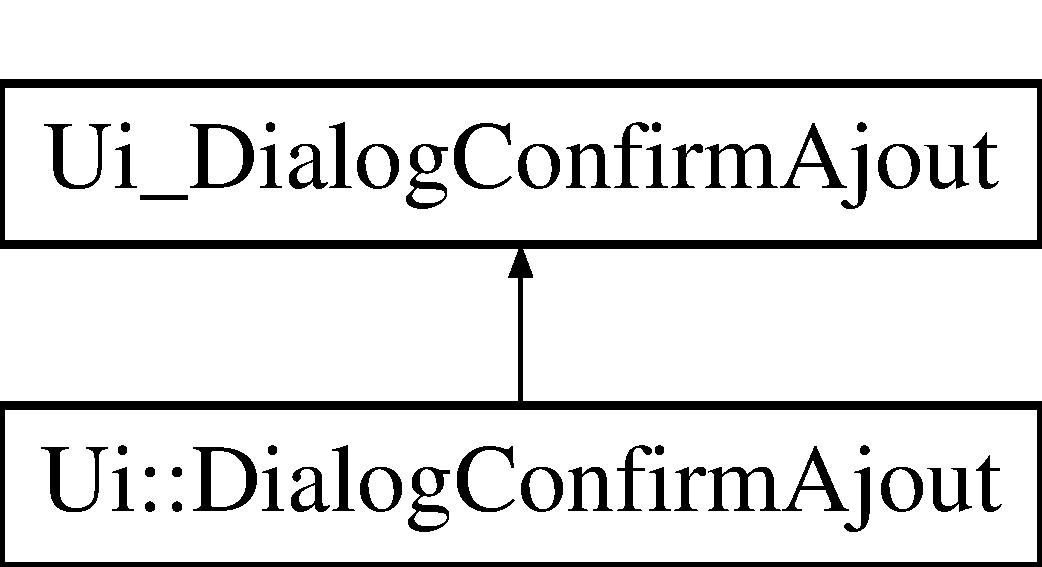
\includegraphics[height=2.000000cm]{classUi__DialogConfirmAjout}
\end{center}
\end{figure}
\subsection*{Public Member Functions}
\begin{DoxyCompactItemize}
\item 
\hypertarget{classUi__DialogConfirmAjout_a2c2e1f935ad91bb607af388752662dcb}{void {\bfseries setup\-Ui} (Q\-Dialog $\ast$\hyperlink{classDialogConfirmAjout}{Dialog\-Confirm\-Ajout})}\label{classUi__DialogConfirmAjout_a2c2e1f935ad91bb607af388752662dcb}

\item 
\hypertarget{classUi__DialogConfirmAjout_a4d7524ac0fda82ac0266539b94d36300}{void {\bfseries retranslate\-Ui} (Q\-Dialog $\ast$\hyperlink{classDialogConfirmAjout}{Dialog\-Confirm\-Ajout})}\label{classUi__DialogConfirmAjout_a4d7524ac0fda82ac0266539b94d36300}

\end{DoxyCompactItemize}
\subsection*{Public Attributes}
\begin{DoxyCompactItemize}
\item 
\hypertarget{classUi__DialogConfirmAjout_a5816c92dd2bf43b51eefe4499e510122}{Q\-Grid\-Layout $\ast$ {\bfseries grid\-Layout}}\label{classUi__DialogConfirmAjout_a5816c92dd2bf43b51eefe4499e510122}

\item 
\hypertarget{classUi__DialogConfirmAjout_a3fb7251cb46f355e3c6def16b3c1bd59}{Q\-V\-Box\-Layout $\ast$ {\bfseries vertical\-Layout\-\_\-2}}\label{classUi__DialogConfirmAjout_a3fb7251cb46f355e3c6def16b3c1bd59}

\item 
\hypertarget{classUi__DialogConfirmAjout_a31b8c7519cd234d8cf7ffd074c9ae3a4}{Q\-V\-Box\-Layout $\ast$ {\bfseries vertical\-Layout}}\label{classUi__DialogConfirmAjout_a31b8c7519cd234d8cf7ffd074c9ae3a4}

\item 
\hypertarget{classUi__DialogConfirmAjout_a9a6fbee8e5492edf2236a36b36999cc1}{Q\-Spacer\-Item $\ast$ {\bfseries vertical\-Spacer}}\label{classUi__DialogConfirmAjout_a9a6fbee8e5492edf2236a36b36999cc1}

\item 
\hypertarget{classUi__DialogConfirmAjout_a41496fce5425add2ac74aed3385d598b}{Q\-H\-Box\-Layout $\ast$ {\bfseries horizontal\-Layout}}\label{classUi__DialogConfirmAjout_a41496fce5425add2ac74aed3385d598b}

\item 
\hypertarget{classUi__DialogConfirmAjout_aa12190760e2a586a2d19824c80ec6f0e}{Q\-Spacer\-Item $\ast$ {\bfseries horizontal\-Spacer}}\label{classUi__DialogConfirmAjout_aa12190760e2a586a2d19824c80ec6f0e}

\item 
\hypertarget{classUi__DialogConfirmAjout_a9d821ec5adae85c1daa31435af7c23dd}{Q\-Label $\ast$ {\bfseries label}}\label{classUi__DialogConfirmAjout_a9d821ec5adae85c1daa31435af7c23dd}

\item 
\hypertarget{classUi__DialogConfirmAjout_af8b05944a613c2e00444ac75d058aaeb}{Q\-Spacer\-Item $\ast$ {\bfseries horizontal\-Spacer\-\_\-2}}\label{classUi__DialogConfirmAjout_af8b05944a613c2e00444ac75d058aaeb}

\item 
\hypertarget{classUi__DialogConfirmAjout_a405e6279388fff2c99144d97d7fd8f33}{Q\-Spacer\-Item $\ast$ {\bfseries vertical\-Spacer\-\_\-2}}\label{classUi__DialogConfirmAjout_a405e6279388fff2c99144d97d7fd8f33}

\item 
\hypertarget{classUi__DialogConfirmAjout_adfa200390347da38f3f484b63ed0d56f}{Q\-H\-Box\-Layout $\ast$ {\bfseries horizontal\-Layout\-\_\-2}}\label{classUi__DialogConfirmAjout_adfa200390347da38f3f484b63ed0d56f}

\item 
\hypertarget{classUi__DialogConfirmAjout_a6d79b56d9e1489f29f758f6badcaf037}{Q\-Spacer\-Item $\ast$ {\bfseries horizontal\-Spacer\-\_\-3}}\label{classUi__DialogConfirmAjout_a6d79b56d9e1489f29f758f6badcaf037}

\item 
\hypertarget{classUi__DialogConfirmAjout_a1b8afe913fcaca4a47045ac4d467acd5}{Q\-Push\-Button $\ast$ {\bfseries push\-Button}}\label{classUi__DialogConfirmAjout_a1b8afe913fcaca4a47045ac4d467acd5}

\end{DoxyCompactItemize}


The documentation for this class was generated from the following file\-:\begin{DoxyCompactItemize}
\item 
ui\-\_\-dialogconfirmajout.\-h\end{DoxyCompactItemize}

\hypertarget{classUi__DialogModifMedicament}{\section{Ui\-\_\-\-Dialog\-Modif\-Medicament Class Reference}
\label{classUi__DialogModifMedicament}\index{Ui\-\_\-\-Dialog\-Modif\-Medicament@{Ui\-\_\-\-Dialog\-Modif\-Medicament}}
}
Inheritance diagram for Ui\-\_\-\-Dialog\-Modif\-Medicament\-:\begin{figure}[H]
\begin{center}
\leavevmode
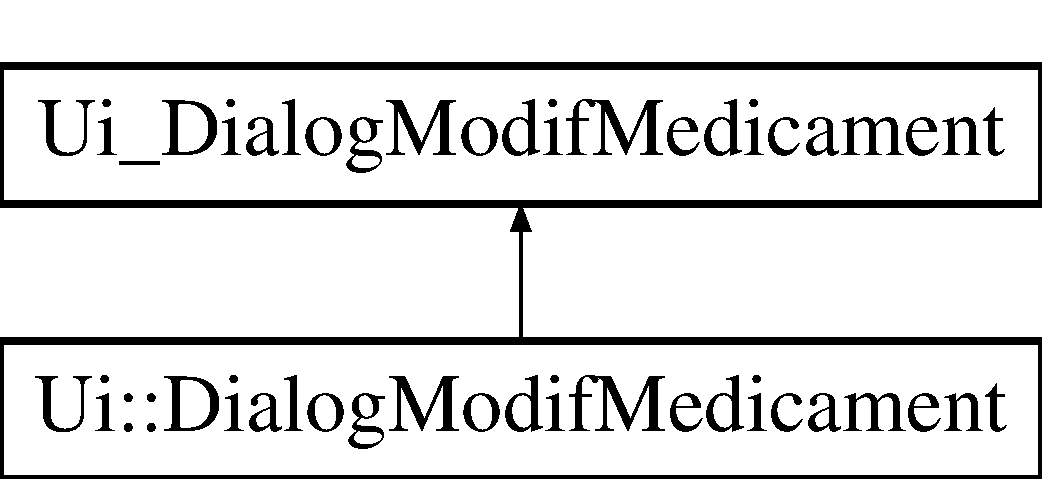
\includegraphics[height=2.000000cm]{classUi__DialogModifMedicament}
\end{center}
\end{figure}
\subsection*{Public Member Functions}
\begin{DoxyCompactItemize}
\item 
\hypertarget{classUi__DialogModifMedicament_adda744bc480f5d83abba8185ee817430}{void {\bfseries setup\-Ui} (Q\-Dialog $\ast$\hyperlink{classDialogModifMedicament}{Dialog\-Modif\-Medicament})}\label{classUi__DialogModifMedicament_adda744bc480f5d83abba8185ee817430}

\item 
\hypertarget{classUi__DialogModifMedicament_af2c1ddb1138afbaf6db6cde652fa2d95}{void {\bfseries retranslate\-Ui} (Q\-Dialog $\ast$\hyperlink{classDialogModifMedicament}{Dialog\-Modif\-Medicament})}\label{classUi__DialogModifMedicament_af2c1ddb1138afbaf6db6cde652fa2d95}

\end{DoxyCompactItemize}
\subsection*{Public Attributes}
\begin{DoxyCompactItemize}
\item 
\hypertarget{classUi__DialogModifMedicament_adaf6df4610fea9c6924b238986ae41a8}{Q\-Grid\-Layout $\ast$ {\bfseries grid\-Layout\-\_\-3}}\label{classUi__DialogModifMedicament_adaf6df4610fea9c6924b238986ae41a8}

\item 
\hypertarget{classUi__DialogModifMedicament_ac40447f78614385dbc6a7d8ffeb20a79}{Q\-V\-Box\-Layout $\ast$ {\bfseries vertical\-Layout\-\_\-6}}\label{classUi__DialogModifMedicament_ac40447f78614385dbc6a7d8ffeb20a79}

\item 
\hypertarget{classUi__DialogModifMedicament_affbf7206b2adf943c31c3b317a1c784d}{Q\-Splitter $\ast$ {\bfseries splitter}}\label{classUi__DialogModifMedicament_affbf7206b2adf943c31c3b317a1c784d}

\item 
\hypertarget{classUi__DialogModifMedicament_aaf652c3b444ff17b4c26bb8e3238820f}{Q\-Widget $\ast$ {\bfseries layout\-Widget}}\label{classUi__DialogModifMedicament_aaf652c3b444ff17b4c26bb8e3238820f}

\item 
\hypertarget{classUi__DialogModifMedicament_aeaca211e93c172403649515deff7f54e}{Q\-V\-Box\-Layout $\ast$ {\bfseries vertical\-Layout\-\_\-5}}\label{classUi__DialogModifMedicament_aeaca211e93c172403649515deff7f54e}

\item 
\hypertarget{classUi__DialogModifMedicament_ac2ae478a22d52c8e00aa1ad2faec6dd9}{Q\-Grid\-Layout $\ast$ {\bfseries grid\-Layout}}\label{classUi__DialogModifMedicament_ac2ae478a22d52c8e00aa1ad2faec6dd9}

\item 
\hypertarget{classUi__DialogModifMedicament_a4d2a54db241d30396265bcb296d6102b}{Q\-Label $\ast$ {\bfseries label}}\label{classUi__DialogModifMedicament_a4d2a54db241d30396265bcb296d6102b}

\item 
\hypertarget{classUi__DialogModifMedicament_a09b31781425f24d449b2dd39ebca4981}{Q\-Line\-Edit $\ast$ {\bfseries line\-Edit\-D\-L}}\label{classUi__DialogModifMedicament_a09b31781425f24d449b2dd39ebca4981}

\item 
\hypertarget{classUi__DialogModifMedicament_a272929578e6ace5f1ec2fb131d7d7715}{Q\-Label $\ast$ {\bfseries label\-\_\-2}}\label{classUi__DialogModifMedicament_a272929578e6ace5f1ec2fb131d7d7715}

\item 
\hypertarget{classUi__DialogModifMedicament_a53a7c17641228c97cc6335b0006b8bd1}{Q\-Line\-Edit $\ast$ {\bfseries line\-Edit\-N\-C}}\label{classUi__DialogModifMedicament_a53a7c17641228c97cc6335b0006b8bd1}

\item 
\hypertarget{classUi__DialogModifMedicament_a56c7576d0c9a33d662cf4fb5a8cdd776}{Q\-Label $\ast$ {\bfseries label\-\_\-3}}\label{classUi__DialogModifMedicament_a56c7576d0c9a33d662cf4fb5a8cdd776}

\item 
\hypertarget{classUi__DialogModifMedicament_a381dd49030ebd0c33de2b2634c74bf76}{Q\-Combo\-Box $\ast$ {\bfseries combo\-Box\-Famille\-Modif}}\label{classUi__DialogModifMedicament_a381dd49030ebd0c33de2b2634c74bf76}

\item 
\hypertarget{classUi__DialogModifMedicament_a2e6fa0485fc381d4e7a0687fe601aa0e}{Q\-Label $\ast$ {\bfseries label\-\_\-4}}\label{classUi__DialogModifMedicament_a2e6fa0485fc381d4e7a0687fe601aa0e}

\item 
\hypertarget{classUi__DialogModifMedicament_ab0b01a8442a3d827da0474b9f49675d2}{Q\-Line\-Edit $\ast$ {\bfseries line\-Edit\-Prix}}\label{classUi__DialogModifMedicament_ab0b01a8442a3d827da0474b9f49675d2}

\item 
\hypertarget{classUi__DialogModifMedicament_aa7b517a771a27a42b90b1f26433b9abc}{Q\-Label $\ast$ {\bfseries label\-\_\-8}}\label{classUi__DialogModifMedicament_aa7b517a771a27a42b90b1f26433b9abc}

\item 
\hypertarget{classUi__DialogModifMedicament_af5452c2adbcbff7a4f6267602b82ce89}{Q\-Widget $\ast$ {\bfseries layout\-Widget1}}\label{classUi__DialogModifMedicament_af5452c2adbcbff7a4f6267602b82ce89}

\item 
\hypertarget{classUi__DialogModifMedicament_a91acbbba34f494db395a6b3b96ed9e23}{Q\-Grid\-Layout $\ast$ {\bfseries grid\-Layout\-\_\-2}}\label{classUi__DialogModifMedicament_a91acbbba34f494db395a6b3b96ed9e23}

\item 
\hypertarget{classUi__DialogModifMedicament_a27df1ad1a34279fd97d2f87b9915fcb0}{Q\-V\-Box\-Layout $\ast$ {\bfseries vertical\-Layout\-\_\-4}}\label{classUi__DialogModifMedicament_a27df1ad1a34279fd97d2f87b9915fcb0}

\item 
\hypertarget{classUi__DialogModifMedicament_afd41812a7e4b93de6d0e63ca79a7e74d}{Q\-V\-Box\-Layout $\ast$ {\bfseries vertical\-Layout}}\label{classUi__DialogModifMedicament_afd41812a7e4b93de6d0e63ca79a7e74d}

\item 
\hypertarget{classUi__DialogModifMedicament_a57afddfde98efe3b9e2552d34522f75b}{Q\-Label $\ast$ {\bfseries label\-\_\-5}}\label{classUi__DialogModifMedicament_a57afddfde98efe3b9e2552d34522f75b}

\item 
\hypertarget{classUi__DialogModifMedicament_a04fd191e7a5d4560466322df4e514c95}{Q\-Spacer\-Item $\ast$ {\bfseries vertical\-Spacer}}\label{classUi__DialogModifMedicament_a04fd191e7a5d4560466322df4e514c95}

\item 
\hypertarget{classUi__DialogModifMedicament_a9165aa41269f481945ef94e0c53dfe36}{Q\-V\-Box\-Layout $\ast$ {\bfseries vertical\-Layout\-\_\-2}}\label{classUi__DialogModifMedicament_a9165aa41269f481945ef94e0c53dfe36}

\item 
\hypertarget{classUi__DialogModifMedicament_acceacf631a3c244a53b56793a00c6b0b}{Q\-Label $\ast$ {\bfseries label\-\_\-6}}\label{classUi__DialogModifMedicament_acceacf631a3c244a53b56793a00c6b0b}

\item 
\hypertarget{classUi__DialogModifMedicament_a75896a7c490d5cef66392b961d2bc25e}{Q\-Spacer\-Item $\ast$ {\bfseries horizontal\-Spacer}}\label{classUi__DialogModifMedicament_a75896a7c490d5cef66392b961d2bc25e}

\item 
\hypertarget{classUi__DialogModifMedicament_af40066c1b11b24b12b44d3b8e5bd3e35}{Q\-Spacer\-Item $\ast$ {\bfseries vertical\-Spacer\-\_\-2}}\label{classUi__DialogModifMedicament_af40066c1b11b24b12b44d3b8e5bd3e35}

\item 
\hypertarget{classUi__DialogModifMedicament_a0bf32eb9f31f21d68a2df55204fb5b4a}{Q\-V\-Box\-Layout $\ast$ {\bfseries vertical\-Layout\-\_\-3}}\label{classUi__DialogModifMedicament_a0bf32eb9f31f21d68a2df55204fb5b4a}

\item 
\hypertarget{classUi__DialogModifMedicament_a4306673ec8015140ccb00d8dc57f2085}{Q\-Label $\ast$ {\bfseries label\-\_\-7}}\label{classUi__DialogModifMedicament_a4306673ec8015140ccb00d8dc57f2085}

\item 
\hypertarget{classUi__DialogModifMedicament_a1ce64e2c297e2ce758f026713614f4a5}{Q\-Spacer\-Item $\ast$ {\bfseries vertical\-Spacer\-\_\-3}}\label{classUi__DialogModifMedicament_a1ce64e2c297e2ce758f026713614f4a5}

\item 
\hypertarget{classUi__DialogModifMedicament_a3c3653f365048fa8cdac98c4afffb174}{Q\-Text\-Edit $\ast$ {\bfseries text\-Edit\-Effets}}\label{classUi__DialogModifMedicament_a3c3653f365048fa8cdac98c4afffb174}

\item 
\hypertarget{classUi__DialogModifMedicament_a3ddc88ec877ecda31826d08a462f1f3a}{Q\-Text\-Edit $\ast$ {\bfseries text\-Edit\-Composition}}\label{classUi__DialogModifMedicament_a3ddc88ec877ecda31826d08a462f1f3a}

\item 
\hypertarget{classUi__DialogModifMedicament_aba758935ccf341a30656900db89c1597}{Q\-Text\-Edit $\ast$ {\bfseries text\-Edit\-C\-I}}\label{classUi__DialogModifMedicament_aba758935ccf341a30656900db89c1597}

\item 
\hypertarget{classUi__DialogModifMedicament_a30dc81e32e379ba3e5ea9a1137e9e4ae}{Q\-H\-Box\-Layout $\ast$ {\bfseries horizontal\-Layout}}\label{classUi__DialogModifMedicament_a30dc81e32e379ba3e5ea9a1137e9e4ae}

\item 
\hypertarget{classUi__DialogModifMedicament_a9385701a9c805b6bcbae4d26f3c663ec}{Q\-Spacer\-Item $\ast$ {\bfseries horizontal\-Spacer\-\_\-2}}\label{classUi__DialogModifMedicament_a9385701a9c805b6bcbae4d26f3c663ec}

\item 
\hypertarget{classUi__DialogModifMedicament_a7a9af19a939de01d66dfea2dd63a7d5b}{Q\-Push\-Button $\ast$ {\bfseries push\-Button\-Ok}}\label{classUi__DialogModifMedicament_a7a9af19a939de01d66dfea2dd63a7d5b}

\item 
\hypertarget{classUi__DialogModifMedicament_a895915fe9da663063de16d09773a2efd}{Q\-Push\-Button $\ast$ {\bfseries push\-Button\-Annuler}}\label{classUi__DialogModifMedicament_a895915fe9da663063de16d09773a2efd}

\end{DoxyCompactItemize}


The documentation for this class was generated from the following file\-:\begin{DoxyCompactItemize}
\item 
ui\-\_\-dialogmodifmedicament.\-h\end{DoxyCompactItemize}

\hypertarget{classUi__DialogModifPraticien}{\section{Ui\-\_\-\-Dialog\-Modif\-Praticien Class Reference}
\label{classUi__DialogModifPraticien}\index{Ui\-\_\-\-Dialog\-Modif\-Praticien@{Ui\-\_\-\-Dialog\-Modif\-Praticien}}
}
Inheritance diagram for Ui\-\_\-\-Dialog\-Modif\-Praticien\-:\begin{figure}[H]
\begin{center}
\leavevmode
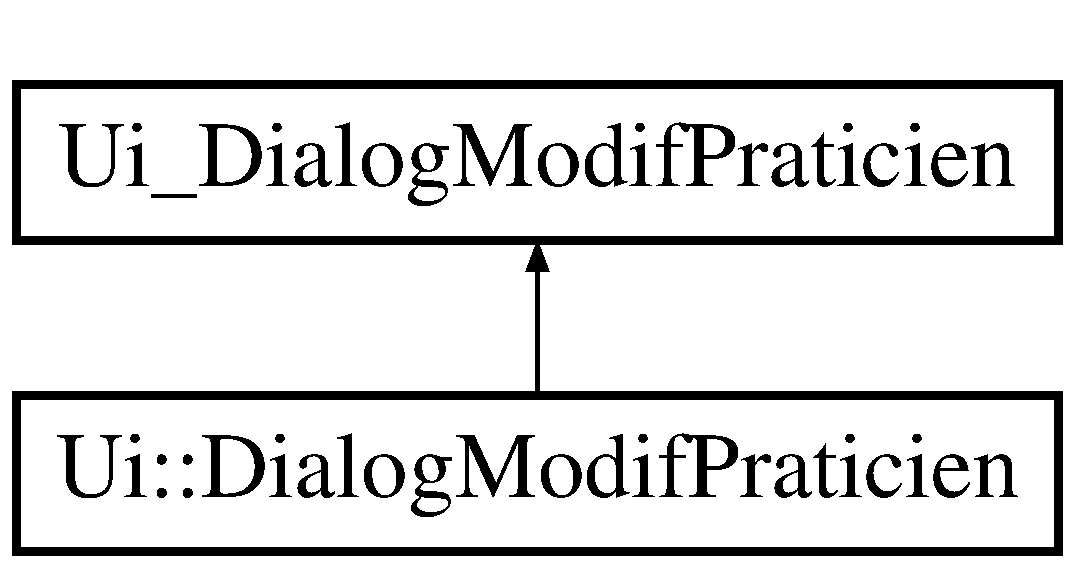
\includegraphics[height=2.000000cm]{classUi__DialogModifPraticien}
\end{center}
\end{figure}
\subsection*{Public Member Functions}
\begin{DoxyCompactItemize}
\item 
\hypertarget{classUi__DialogModifPraticien_aa39e1af2907fb461561a6f664c27552f}{void {\bfseries setup\-Ui} (Q\-Dialog $\ast$\hyperlink{classDialogModifPraticien}{Dialog\-Modif\-Praticien})}\label{classUi__DialogModifPraticien_aa39e1af2907fb461561a6f664c27552f}

\item 
\hypertarget{classUi__DialogModifPraticien_ac74eb93817e43dccd056b77add66dbf6}{void {\bfseries retranslate\-Ui} (Q\-Dialog $\ast$\hyperlink{classDialogModifPraticien}{Dialog\-Modif\-Praticien})}\label{classUi__DialogModifPraticien_ac74eb93817e43dccd056b77add66dbf6}

\end{DoxyCompactItemize}
\subsection*{Public Attributes}
\begin{DoxyCompactItemize}
\item 
\hypertarget{classUi__DialogModifPraticien_a3e1229720cc3b9f35ef98653c519dd6b}{Q\-V\-Box\-Layout $\ast$ {\bfseries vertical\-Layout}}\label{classUi__DialogModifPraticien_a3e1229720cc3b9f35ef98653c519dd6b}

\item 
\hypertarget{classUi__DialogModifPraticien_a022dada4160784345c6ed6a27be91caa}{Q\-H\-Box\-Layout $\ast$ {\bfseries horizontal\-Layout\-\_\-2}}\label{classUi__DialogModifPraticien_a022dada4160784345c6ed6a27be91caa}

\item 
\hypertarget{classUi__DialogModifPraticien_a5bfc0735c62a8db462a5a48f9133fd3c}{Q\-Spacer\-Item $\ast$ {\bfseries horizontal\-Spacer\-\_\-2}}\label{classUi__DialogModifPraticien_a5bfc0735c62a8db462a5a48f9133fd3c}

\item 
\hypertarget{classUi__DialogModifPraticien_a9e69b65b119c7f4714886d64b0040a1b}{Q\-Grid\-Layout $\ast$ {\bfseries grid\-Layout}}\label{classUi__DialogModifPraticien_a9e69b65b119c7f4714886d64b0040a1b}

\item 
\hypertarget{classUi__DialogModifPraticien_ac2ca21500fb6c592b7609e66ecf8c222}{Q\-Label $\ast$ {\bfseries label}}\label{classUi__DialogModifPraticien_ac2ca21500fb6c592b7609e66ecf8c222}

\item 
\hypertarget{classUi__DialogModifPraticien_a6999cd3fd90ffce90a5fe3ef6ba85f33}{Q\-Line\-Edit $\ast$ {\bfseries line\-Edit\-Matricule}}\label{classUi__DialogModifPraticien_a6999cd3fd90ffce90a5fe3ef6ba85f33}

\item 
\hypertarget{classUi__DialogModifPraticien_aff7b55b09db05bc1cff56cbeecb79f7c}{Q\-Label $\ast$ {\bfseries label\-\_\-2}}\label{classUi__DialogModifPraticien_aff7b55b09db05bc1cff56cbeecb79f7c}

\item 
\hypertarget{classUi__DialogModifPraticien_ac0d6552243e2d84b968505072aba6a93}{Q\-Line\-Edit $\ast$ {\bfseries line\-Edit\-Nom}}\label{classUi__DialogModifPraticien_ac0d6552243e2d84b968505072aba6a93}

\item 
\hypertarget{classUi__DialogModifPraticien_ae73ee2f204aba6217e8c96027f70bbe3}{Q\-Label $\ast$ {\bfseries label\-\_\-3}}\label{classUi__DialogModifPraticien_ae73ee2f204aba6217e8c96027f70bbe3}

\item 
\hypertarget{classUi__DialogModifPraticien_ab70cdd4783071bb0fd09bf1141d15f11}{Q\-Line\-Edit $\ast$ {\bfseries line\-Edit\-Prenom}}\label{classUi__DialogModifPraticien_ab70cdd4783071bb0fd09bf1141d15f11}

\item 
\hypertarget{classUi__DialogModifPraticien_a9bd91d274024034c95914e769aa3e9df}{Q\-Label $\ast$ {\bfseries label\-\_\-4}}\label{classUi__DialogModifPraticien_a9bd91d274024034c95914e769aa3e9df}

\item 
\hypertarget{classUi__DialogModifPraticien_a7ad3246b26f689faf9a38ac020ee6658}{Q\-Line\-Edit $\ast$ {\bfseries line\-Edit\-Adresse}}\label{classUi__DialogModifPraticien_a7ad3246b26f689faf9a38ac020ee6658}

\item 
\hypertarget{classUi__DialogModifPraticien_a01e1b3b6de02bada0c9dabc90a48fea3}{Q\-Label $\ast$ {\bfseries label\-\_\-5}}\label{classUi__DialogModifPraticien_a01e1b3b6de02bada0c9dabc90a48fea3}

\item 
\hypertarget{classUi__DialogModifPraticien_a8c2f1018ec77b5d992776df16516367b}{Q\-Line\-Edit $\ast$ {\bfseries line\-Edit\-C\-P}}\label{classUi__DialogModifPraticien_a8c2f1018ec77b5d992776df16516367b}

\item 
\hypertarget{classUi__DialogModifPraticien_a6620795e281b63a9627c76af2cfb3d24}{Q\-Label $\ast$ {\bfseries label\-\_\-6}}\label{classUi__DialogModifPraticien_a6620795e281b63a9627c76af2cfb3d24}

\item 
\hypertarget{classUi__DialogModifPraticien_a0aa86b6ffebccfd81e1b161ac4a9ace1}{Q\-Line\-Edit $\ast$ {\bfseries line\-Edit\-Ville}}\label{classUi__DialogModifPraticien_a0aa86b6ffebccfd81e1b161ac4a9ace1}

\item 
\hypertarget{classUi__DialogModifPraticien_a82c4ddbe5210e79f09e6bdb711922611}{Q\-Label $\ast$ {\bfseries label\-\_\-7}}\label{classUi__DialogModifPraticien_a82c4ddbe5210e79f09e6bdb711922611}

\item 
\hypertarget{classUi__DialogModifPraticien_a2ebcbb41d432d73f27adc89e4f080804}{Q\-Label $\ast$ {\bfseries label\-\_\-8}}\label{classUi__DialogModifPraticien_a2ebcbb41d432d73f27adc89e4f080804}

\item 
\hypertarget{classUi__DialogModifPraticien_aa491d31af864717682e5442be17b82bc}{Q\-Combo\-Box $\ast$ {\bfseries combo\-Box\-Type\-Modif}}\label{classUi__DialogModifPraticien_aa491d31af864717682e5442be17b82bc}

\item 
\hypertarget{classUi__DialogModifPraticien_a3838b5bd798f8106fcd7fd87ec67278e}{Q\-Line\-Edit $\ast$ {\bfseries line\-Edit\-C\-N}}\label{classUi__DialogModifPraticien_a3838b5bd798f8106fcd7fd87ec67278e}

\item 
\hypertarget{classUi__DialogModifPraticien_af7399b57f1024452ad570a04548b6673}{Q\-Spacer\-Item $\ast$ {\bfseries horizontal\-Spacer\-\_\-3}}\label{classUi__DialogModifPraticien_af7399b57f1024452ad570a04548b6673}

\item 
\hypertarget{classUi__DialogModifPraticien_a288ed93851e180702fddd74ac6d263d3}{Q\-H\-Box\-Layout $\ast$ {\bfseries horizontal\-Layout}}\label{classUi__DialogModifPraticien_a288ed93851e180702fddd74ac6d263d3}

\item 
\hypertarget{classUi__DialogModifPraticien_a635125f62494b287a2abebc4f0243264}{Q\-Spacer\-Item $\ast$ {\bfseries horizontal\-Spacer}}\label{classUi__DialogModifPraticien_a635125f62494b287a2abebc4f0243264}

\item 
\hypertarget{classUi__DialogModifPraticien_afb0bf0a7336b5f19b6a11fb881573ffa}{Q\-Push\-Button $\ast$ {\bfseries push\-Button\-Ok}}\label{classUi__DialogModifPraticien_afb0bf0a7336b5f19b6a11fb881573ffa}

\item 
\hypertarget{classUi__DialogModifPraticien_a7902da557540de676f5c939a907be786}{Q\-Push\-Button $\ast$ {\bfseries push\-Button\-Annuler}}\label{classUi__DialogModifPraticien_a7902da557540de676f5c939a907be786}

\end{DoxyCompactItemize}


The documentation for this class was generated from the following file\-:\begin{DoxyCompactItemize}
\item 
ui\-\_\-dialogmodifpraticien.\-h\end{DoxyCompactItemize}

\hypertarget{classUi__MainWindow}{\section{Ui\-\_\-\-Main\-Window Class Reference}
\label{classUi__MainWindow}\index{Ui\-\_\-\-Main\-Window@{Ui\-\_\-\-Main\-Window}}
}
Inheritance diagram for Ui\-\_\-\-Main\-Window\-:\begin{figure}[H]
\begin{center}
\leavevmode
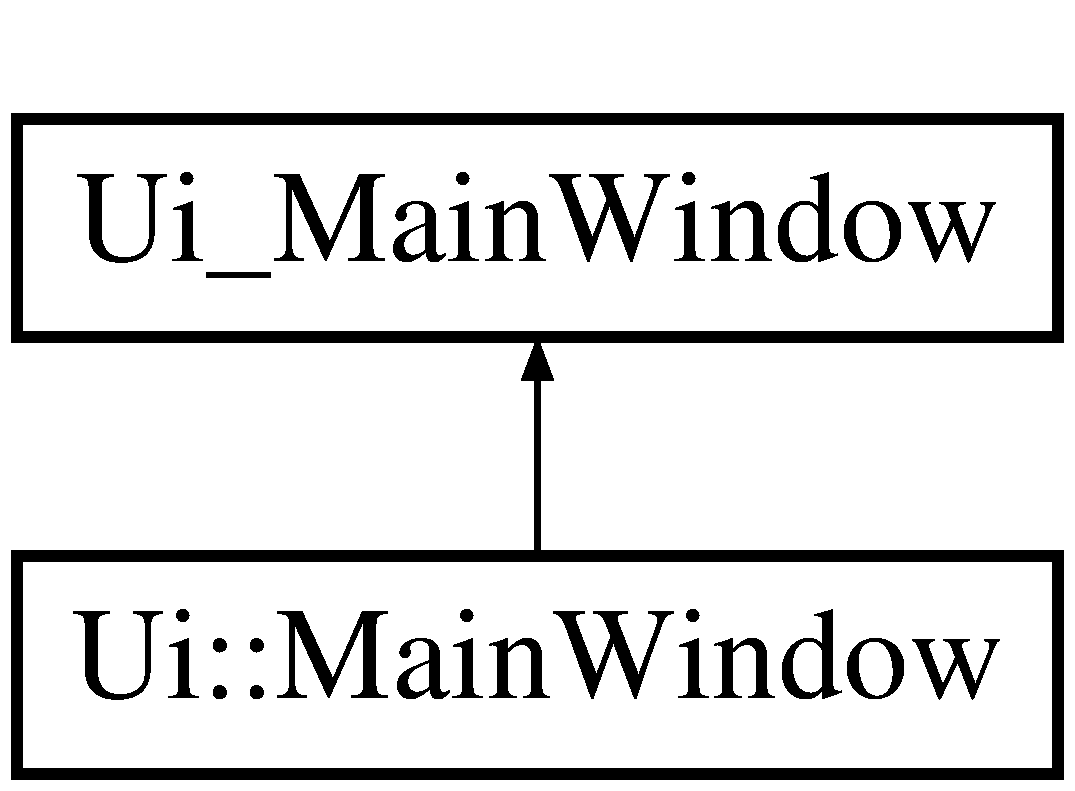
\includegraphics[height=2.000000cm]{classUi__MainWindow}
\end{center}
\end{figure}
\subsection*{Public Member Functions}
\begin{DoxyCompactItemize}
\item 
\hypertarget{classUi__MainWindow_acf4a0872c4c77d8f43a2ec66ed849b58}{void {\bfseries setup\-Ui} (Q\-Main\-Window $\ast$\hyperlink{classMainWindow}{Main\-Window})}\label{classUi__MainWindow_acf4a0872c4c77d8f43a2ec66ed849b58}

\item 
\hypertarget{classUi__MainWindow_a097dd160c3534a204904cb374412c618}{void {\bfseries retranslate\-Ui} (Q\-Main\-Window $\ast$\hyperlink{classMainWindow}{Main\-Window})}\label{classUi__MainWindow_a097dd160c3534a204904cb374412c618}

\end{DoxyCompactItemize}
\subsection*{Public Attributes}
\begin{DoxyCompactItemize}
\item 
\hypertarget{classUi__MainWindow_a16d39d241a02bfb61fab07149d15868f}{Q\-Action $\ast$ {\bfseries action\-\_\-\-Quitter}}\label{classUi__MainWindow_a16d39d241a02bfb61fab07149d15868f}

\item 
\hypertarget{classUi__MainWindow_a7699b501da4a634d45a4b8887ad17dbb}{Q\-Action $\ast$ {\bfseries action\-\_\-\-Changer\-\_\-d\-\_\-utilisateur}}\label{classUi__MainWindow_a7699b501da4a634d45a4b8887ad17dbb}

\item 
\hypertarget{classUi__MainWindow_a30075506c2116c3ed4ff25e07ae75f81}{Q\-Widget $\ast$ {\bfseries central\-Widget}}\label{classUi__MainWindow_a30075506c2116c3ed4ff25e07ae75f81}

\item 
\hypertarget{classUi__MainWindow_a6b2a0c5f7e8ff2a87134908dd770d2d2}{Q\-Grid\-Layout $\ast$ {\bfseries grid\-Layout\-\_\-2}}\label{classUi__MainWindow_a6b2a0c5f7e8ff2a87134908dd770d2d2}

\item 
\hypertarget{classUi__MainWindow_a525ed3c5fe0784ac502ee222fba4e205}{Q\-Grid\-Layout $\ast$ {\bfseries grid\-Layout}}\label{classUi__MainWindow_a525ed3c5fe0784ac502ee222fba4e205}

\item 
\hypertarget{classUi__MainWindow_a3260b943854b841c986f47c4726ee7f9}{Q\-Tab\-Widget $\ast$ {\bfseries tab\-Widget}}\label{classUi__MainWindow_a3260b943854b841c986f47c4726ee7f9}

\item 
\hypertarget{classUi__MainWindow_a3efc28c664e9f5115095aafbbc5ac6bc}{Q\-Widget $\ast$ {\bfseries tab}}\label{classUi__MainWindow_a3efc28c664e9f5115095aafbbc5ac6bc}

\item 
\hypertarget{classUi__MainWindow_af42ea7d4c2e893181caad21e28166932}{Q\-Grid\-Layout $\ast$ {\bfseries grid\-Layout\-\_\-3}}\label{classUi__MainWindow_af42ea7d4c2e893181caad21e28166932}

\item 
\hypertarget{classUi__MainWindow_aecd96a04789fcfec3f98d80390ad8184}{Q\-V\-Box\-Layout $\ast$ {\bfseries vertical\-Layout}}\label{classUi__MainWindow_aecd96a04789fcfec3f98d80390ad8184}

\item 
\hypertarget{classUi__MainWindow_acd6fdc9ebacc4b25b834162380d75ce8}{Q\-H\-Box\-Layout $\ast$ {\bfseries horizontal\-Layout}}\label{classUi__MainWindow_acd6fdc9ebacc4b25b834162380d75ce8}

\item 
\hypertarget{classUi__MainWindow_a2e2516d755e4dd53fc905dabddf2738a}{Q\-Label $\ast$ {\bfseries label\-\_\-2}}\label{classUi__MainWindow_a2e2516d755e4dd53fc905dabddf2738a}

\item 
\hypertarget{classUi__MainWindow_a224d366a76eb05bb5b7fa020f5b9dbb1}{Q\-Combo\-Box $\ast$ {\bfseries combo\-Box\-Famille\-Main}}\label{classUi__MainWindow_a224d366a76eb05bb5b7fa020f5b9dbb1}

\item 
\hypertarget{classUi__MainWindow_a3a90f6631359f1f32a482b0df51617ef}{Q\-List\-Widget $\ast$ {\bfseries list\-Widget\-Medicament}}\label{classUi__MainWindow_a3a90f6631359f1f32a482b0df51617ef}

\item 
\hypertarget{classUi__MainWindow_a80867018070156432923d0266cc9fe25}{Q\-H\-Box\-Layout $\ast$ {\bfseries horizontal\-Layout\-\_\-2}}\label{classUi__MainWindow_a80867018070156432923d0266cc9fe25}

\item 
\hypertarget{classUi__MainWindow_a10f036266abf36062ce6b983dd25615d}{Q\-Push\-Button $\ast$ {\bfseries push\-Button\-Ajout\-Medicament}}\label{classUi__MainWindow_a10f036266abf36062ce6b983dd25615d}

\item 
\hypertarget{classUi__MainWindow_a2fdc675a714e0cf6e9ab3c44a9410022}{Q\-Push\-Button $\ast$ {\bfseries push\-Button\-Modif\-Medicament}}\label{classUi__MainWindow_a2fdc675a714e0cf6e9ab3c44a9410022}

\item 
\hypertarget{classUi__MainWindow_a397e9b4283f7bf302dd0ec9f3844229b}{Q\-Push\-Button $\ast$ {\bfseries push\-Button\-Supp\-Medicament}}\label{classUi__MainWindow_a397e9b4283f7bf302dd0ec9f3844229b}

\item 
\hypertarget{classUi__MainWindow_a83495b23cbc6810f81978dc0d584b810}{Q\-Widget $\ast$ {\bfseries tab\-\_\-2}}\label{classUi__MainWindow_a83495b23cbc6810f81978dc0d584b810}

\item 
\hypertarget{classUi__MainWindow_a8ee86315639f324b17708efc7dbe8b19}{Q\-Grid\-Layout $\ast$ {\bfseries grid\-Layout\-\_\-4}}\label{classUi__MainWindow_a8ee86315639f324b17708efc7dbe8b19}

\item 
\hypertarget{classUi__MainWindow_a8ead8fc876ee91c30864822eedb9c370}{Q\-H\-Box\-Layout $\ast$ {\bfseries horizontal\-Layout\-\_\-8}}\label{classUi__MainWindow_a8ead8fc876ee91c30864822eedb9c370}

\item 
\hypertarget{classUi__MainWindow_ae183387a7d233b437a637b403ba39ffd}{Q\-H\-Box\-Layout $\ast$ {\bfseries horizontal\-Layout\-\_\-4}}\label{classUi__MainWindow_ae183387a7d233b437a637b403ba39ffd}

\item 
\hypertarget{classUi__MainWindow_a78c7e10730b43c6700cd7216911ed76a}{Q\-Label $\ast$ {\bfseries label\-\_\-4}}\label{classUi__MainWindow_a78c7e10730b43c6700cd7216911ed76a}

\item 
\hypertarget{classUi__MainWindow_a0622c68d3396a7bf6c350a2b436da014}{Q\-Combo\-Box $\ast$ {\bfseries combo\-Box\-Ville}}\label{classUi__MainWindow_a0622c68d3396a7bf6c350a2b436da014}

\item 
\hypertarget{classUi__MainWindow_a2afb915e1492b7e6704db4918c1e5e80}{Q\-H\-Box\-Layout $\ast$ {\bfseries horizontal\-Layout\-\_\-7}}\label{classUi__MainWindow_a2afb915e1492b7e6704db4918c1e5e80}

\item 
\hypertarget{classUi__MainWindow_ad9c89133780f28e6efa2ec17ceb9cff5}{Q\-Label $\ast$ {\bfseries label}}\label{classUi__MainWindow_ad9c89133780f28e6efa2ec17ceb9cff5}

\item 
\hypertarget{classUi__MainWindow_a8864cf9be266b0de14c7f1da90376c77}{Q\-Combo\-Box $\ast$ {\bfseries combo\-Box\-Type}}\label{classUi__MainWindow_a8864cf9be266b0de14c7f1da90376c77}

\item 
\hypertarget{classUi__MainWindow_a416699fb8ee351e3970d47a6aee6a86f}{Q\-List\-Widget $\ast$ {\bfseries list\-Widget\-Praticien}}\label{classUi__MainWindow_a416699fb8ee351e3970d47a6aee6a86f}

\item 
\hypertarget{classUi__MainWindow_a03ce63974cc69b067c91bbf285cceca8}{Q\-H\-Box\-Layout $\ast$ {\bfseries horizontal\-Layout\-\_\-3}}\label{classUi__MainWindow_a03ce63974cc69b067c91bbf285cceca8}

\item 
\hypertarget{classUi__MainWindow_ac3f16a152c2843e7dd421f7c4a25d64d}{Q\-Push\-Button $\ast$ {\bfseries push\-Button\-Ajout\-Praticien}}\label{classUi__MainWindow_ac3f16a152c2843e7dd421f7c4a25d64d}

\item 
\hypertarget{classUi__MainWindow_a0108696055b1d904392f786189b72f24}{Q\-Push\-Button $\ast$ {\bfseries push\-Button\-Modif\-Praticien}}\label{classUi__MainWindow_a0108696055b1d904392f786189b72f24}

\item 
\hypertarget{classUi__MainWindow_a0df202c7a836fece1576489a5d170e0e}{Q\-Push\-Button $\ast$ {\bfseries push\-Button\-Supp\-Praticien}}\label{classUi__MainWindow_a0df202c7a836fece1576489a5d170e0e}

\item 
\hypertarget{classUi__MainWindow_a41c7e77dd12b9445e13dbe8fb5ae1488}{Q\-Widget $\ast$ {\bfseries tab\-\_\-3}}\label{classUi__MainWindow_a41c7e77dd12b9445e13dbe8fb5ae1488}

\item 
\hypertarget{classUi__MainWindow_a8731b71c513ff94baf59614807823c5d}{Q\-Grid\-Layout $\ast$ {\bfseries grid\-Layout\-\_\-5}}\label{classUi__MainWindow_a8731b71c513ff94baf59614807823c5d}

\item 
\hypertarget{classUi__MainWindow_a14c9d4842c3e97e16e7873ef0aecdb1e}{Q\-H\-Box\-Layout $\ast$ {\bfseries horizontal\-Layout\-\_\-5}}\label{classUi__MainWindow_a14c9d4842c3e97e16e7873ef0aecdb1e}

\item 
\hypertarget{classUi__MainWindow_a0376fd90247280e7c7957cc70628708c}{Q\-Label $\ast$ {\bfseries label\-\_\-3}}\label{classUi__MainWindow_a0376fd90247280e7c7957cc70628708c}

\item 
\hypertarget{classUi__MainWindow_a048d3f935a966a97e10e122cb4f5b18c}{Q\-Combo\-Box $\ast$ {\bfseries combo\-Box\-Ville2}}\label{classUi__MainWindow_a048d3f935a966a97e10e122cb4f5b18c}

\item 
\hypertarget{classUi__MainWindow_afb925f4fee1eccabbcf71e8a2523aca9}{Q\-List\-Widget $\ast$ {\bfseries list\-Widget\-Visiteur}}\label{classUi__MainWindow_afb925f4fee1eccabbcf71e8a2523aca9}

\item 
\hypertarget{classUi__MainWindow_a1351e317cba7ca711b6b4d2212b6bf36}{Q\-H\-Box\-Layout $\ast$ {\bfseries horizontal\-Layout\-\_\-6}}\label{classUi__MainWindow_a1351e317cba7ca711b6b4d2212b6bf36}

\item 
\hypertarget{classUi__MainWindow_a016864ffa110d63b5c6a9208b9e787ed}{Q\-Push\-Button $\ast$ {\bfseries push\-Button\-Ajout\-Visiteur}}\label{classUi__MainWindow_a016864ffa110d63b5c6a9208b9e787ed}

\item 
\hypertarget{classUi__MainWindow_af8173b0d70f790869d1b04f19059fefe}{Q\-Push\-Button $\ast$ {\bfseries push\-Button\-Modif\-Visiteur}}\label{classUi__MainWindow_af8173b0d70f790869d1b04f19059fefe}

\item 
\hypertarget{classUi__MainWindow_a0856850158021cdb9f294cbc8b323bc8}{Q\-Push\-Button $\ast$ {\bfseries push\-Button\-Supp\-Visiteur}}\label{classUi__MainWindow_a0856850158021cdb9f294cbc8b323bc8}

\item 
\hypertarget{classUi__MainWindow_a2be1c24ec9adfca18e1dcc951931457f}{Q\-Menu\-Bar $\ast$ {\bfseries menu\-Bar}}\label{classUi__MainWindow_a2be1c24ec9adfca18e1dcc951931457f}

\item 
\hypertarget{classUi__MainWindow_a073cce6e21486d944090502ae6949476}{Q\-Menu $\ast$ {\bfseries menu\-\_\-\-Fichier}}\label{classUi__MainWindow_a073cce6e21486d944090502ae6949476}

\item 
\hypertarget{classUi__MainWindow_a5172877001c8c7b4e0f6de50421867d1}{Q\-Tool\-Bar $\ast$ {\bfseries main\-Tool\-Bar}}\label{classUi__MainWindow_a5172877001c8c7b4e0f6de50421867d1}

\item 
\hypertarget{classUi__MainWindow_a50fa481337604bcc8bf68de18ab16ecd}{Q\-Status\-Bar $\ast$ {\bfseries status\-Bar}}\label{classUi__MainWindow_a50fa481337604bcc8bf68de18ab16ecd}

\end{DoxyCompactItemize}


The documentation for this class was generated from the following file\-:\begin{DoxyCompactItemize}
\item 
ui\-\_\-mainwindow.\-h\end{DoxyCompactItemize}

\printindex
\end{document}
